\documentclass[conference]{IEEEtran}
%% SECON 2013 addition:
\makeatletter
\def\ps@headings{%
\def\@oddhead{\mbox{}\scriptsize\rightmark \hfil \thepage}%
\def\@evenhead{\scriptsize\thepage \hfil \leftmark\mbox{}}%
\def\@oddfoot{}%
\def\@evenfoot{}}
\makeatother
\pagestyle{headings} 

\ifCLASSINFOpdf
  % \usepackage[pdftex]{graphicx}
  % declare the path(s) where your graphic files are
  % \graphicspath{{../pdf/}{../jpeg/}}
  % and their extensions so you won't have to specify these with
  % every instance of \includegraphics
  % \DeclareGraphicsExtensions{.pdf,.jpeg,.png}
\else
  % or other class option (dvipsone, dvipdf, if not using dvips). graphicx
  % will default to the driver specified in the system graphics.cfg if no
  % driver is specified.
  % \usepackage[dvips]{graphicx}
  % declare the path(s) where your graphic files are
  % \graphicspath{{../eps/}}
  % and their extensions so you won't have to specify these with
  % every instance of \includegraphics
  % \DeclareGraphicsExtensions{.eps}
\fi
% *** MATH PACKAGES ***
%
\usepackage[cmex10]{amsmath}
\usepackage{amsfonts}
\usepackage{graphicx, epsfig}
\usepackage{color}
\usepackage{subfigure}
\usepackage{xspace}
\usepackage{algorithm}
\usepackage{algpseudocode}
\usepackage{breqn}
\usepackage{cite}
\usepackage{url}
\usepackage[export]{adjustbox}
%\usepackage[bottom]{footmisc}
\raggedbottom

\renewcommand{\thealgorithm}{}
\algnewcommand{\LineComment}[1]{\State \(\triangleright\) #1}
% A popular package from the American Mathematical Society that provides
% many useful and powerful commands for dealing with mathematics. If using
% it, be sure to load this package with the cmex10 option to ensure that
% only type 1 fonts will utilized at all point sizes. Without this option,
% it is possible that some math symbols, particularly those within
% footnotes, will be rendered in bitmap form which will result in a
% document that can not be IEEE Xplore compliant!
%
%\usepackage{array}
%\usepackage{mdwmath}
%\usepackage{mdwtab}
%\usepackage{eqparbox}
%\usepackage[tight,footnotesize]{subfigure}
%\usepackage[caption=false]{caption}
%\usepackage[font=footnotesize]{subfig}
%\usepackage[caption=false,font=footnotesize]{subfig}
%
%\usepackage{fixltx2e}

%\usepackage{stfloats}

%\usepackage{url}

\usepackage[margin=0.8in]{geometry}
\addtolength{\topmargin}{0.25in}

% correct bad hyphenation here
\hyphenation{net-works}

\DeclareMathOperator*{\E}{\mathbb{E}}

\begin{document}
%
% paper title
% can use linebreaks \\ within to get better formatting as desired
\title{Scalability and Satisfiability of Quality-of-Information in Wireless Networks}

\IEEEoverridecommandlockouts

% author names and affiliations
% use a multiple column layout for up to three different
% affiliations

%\author{\IEEEauthorblockN{Scott Rager}
%\IEEEauthorblockA{Department of Computer Science and Engineering\\
%Pennsylvania State University\\
%University Park, PA 16802\\
%Email: rager@psu.edu}}

%\author{\IEEEauthorblockN{Scott Rager, Ertugrul Ciftcioglu, Thomas La Porta}
%\IEEEauthorblockA{Department of Computer Science\\
%and Engineering\\
%Pennsylvania State University\\
%University Park, PA 16802\\
%Email: rager@psu.edu, enc118@psu.edu, tlp@cse.psu.edu}
%\and
%\IEEEauthorblockN{Alice Leung, William Dron}
%\IEEEauthorblockA{Raytheon BBN Technologies\\
%Cambridge, MA 02138\\
%Email: aleung@bbn.com, wdron@bbn.com}
%\and
%\IEEEauthorblockN{John Hancock}
%\IEEEauthorblockA{Artistech\\
%City, State Zip Code\\
%Email: johnh@artistech.com}
%}

\author{
  \IEEEauthorblockN{Scott T. Rager\IEEEauthorrefmark{1} \quad Ertugrul N. Ciftcioglu\IEEEauthorrefmark{2}  \quad Ram Ramanathan\IEEEauthorrefmark{3} \quad Thomas F. La Porta\IEEEauthorrefmark{1} \quad Ramesh Govindan\IEEEauthorrefmark{4} \\
  }
  \IEEEauthorblockA{
  	\IEEEauthorrefmark{1}The Pennsylvania State University, University Park, PA 16802\\
	\IEEEauthorrefmark{2}IBM Research, Yorktown Heights, NY 10598 \\
  \IEEEauthorrefmark{3}Raytheon BBN Technologies, Cambridge, MA 02138 \\
  \IEEEauthorrefmark{4}University of Southern California, Los Angeles, CA 90089
  }

  Email:  rager@psu.edu, enciftci@us.ibm.com , ramanath@bbn.com, tlp@cse.psu.edu, ramesh@usc.edu
\thanks{Research was sponsored by the U.S. Army Research Laboratory under the Network Science Collaborative Technology Alliance, Agreement Number W911NF-09-2-0053. } 
}


% for over three affiliations, or if they all won't fit within the width
% of the page, use this alternative format:
% 
%\author{\IEEEauthorblockN{Michael Shell\IEEEauthorrefmark{1},
%Homer Simpson\IEEEauthorrefmark{2},
%James Kirk\IEEEauthorrefmark{3}, 
%Montgomery Scott\IEEEauthorrefmark{3} and
%Eldon Tyrell\IEEEauthorrefmark{4}}
%\IEEEauthorblockA{\IEEEauthorrefmark{1}School of Electrical and Computer Engineering\\
%Georgia Institute of Technology,
%Atlanta, Georgia 30332--0250\\ Email: see http://www.michaelshell.org/contact.html}
%\IEEEauthorblockA{\IEEEauthorrefmark{2}Twentieth Century Fox, Springfield, USA\\
%Email: homer@thesimpsons.com}
%\IEEEauthorblockA{\IEEEauthorrefmark{3}Starfleet Academy, San Francisco, California 96678-2391\\
%Telephone: (800) 555--1212, Fax: (888) 555--1212}
%\IEEEauthorblockA{\IEEEauthorrefmark{4}Tyrell Inc., 123 Replicant Street, Los Angeles, California 90210--4321}}



% use for special paper notices
%\IEEEspecialpapernotice{(Invited Paper)}




% make the title area
\maketitle


\begin{abstract}
\boldmath
%area
%problem
Quality of Information (QoI) provides a context-dependent measure of the utility that a network delivers to its users by incorporating non-traditional information attributes.  
Quickly and easily predicting performance and limitations of a network using QoI metrics is a valuable tool for network design and deployment. Even more useful is an understanding of how network components like topology, bandwidth, protocols, etc. impact these limitations. 
%solution
In this paper, we develop a QoI-based framework that can be used to provide this understanding of limitations and impact by modeling the various contributors to delay in the network, including channel rate and contention, competing traffic flows, and multi-hop propagation effects, and relating them to QoI requirements, especially completeness and timeliness.
%results
Analysis shows that large tradeoffs exist between different network parameters, such as QoI requirements, topology, and network size.  Simulation results also provide evidence that the developed framework can estimate network limits with high accuracy.  Finally, this work also introduces and shows an example of \emph{scalably feasible QoI regions}, which provide upper bounds on QoI requirements that can be supported for certain network applications.
%takeaway


\end{abstract}

% IEEEtran.cls defaults to using nonbold math in the Abstract.
% This preserves the distinction between vectors and scalars. However,
% if the conference you are submitting to favors bold math in the abstract,
% then you can use LaTeX's standard command \boldmath at the very start
% of the abstract to achieve this. Many IEEE journals/conferences frown on
% math in the abstract anyway.

% no keywords




% For peer review papers, you can put extra information on the cover
% page as needed:
% \ifCLASSOPTIONpeerreview
% \begin{center} \bfseries EDICS Category: 3-BBND \end{center}
% \fi
%
% For peerreview papers, this IEEEtran command inserts a page break and
% creates the second title. It will be ignored for other modes.
\IEEEpeerreviewmaketitle


\section{Introduction}
\label{sec:intro}

%area
Symptotic analysis is an emerging field of characterizing practical network scalability instead of the common asymptotic analysis.  Introduced in \cite{scalability_manets_theory_vs_practice}, symptotics is extremely useful for applications and network designers that are interested in determining the limits of a specific network implementation as well as how various factors affect these limits in terms of scalability.  For example, if one is designing an emergency mesh network to quickly install to replace destroyed infrastructure after a natural disaster, understanding the traffic limitations or what topology allows for the largest feasible network size is crucial to successful design.

%problem
%why not solved
While including the consideration of Quality of Information (QoI) into network control protocols or analysis is not novel, its limitations and effects on network scalability have not been considered before.  This consideration is extremely important, though, because in many recent fields of study, QoI is being used as the metric of a network's capabilities.  Increasingly, network nodes are becoming more capable of affecting QoI through data fusion, compression, selection, etc.  This work aims to begin understanding the connections between these actions and practical network scalability.

%insight
Specifically, in this work we consider the practical effects of real networks as protocol overhead, contention, rates in conjunction with QoI.  While adopting a general framework for QoI, we use timely, similarity-based image collection to provide motivation and concrete applications with results.  

%contribution
Our results first provide maximum sizes to which the networks can scale, given requested levels of QoI. The QoI depends on timeliness and one of two metrics considered: completeness or diversity.  These attributes are defined by the sum similarity of collected images resulting from Top-K queries for completeness, and sum dissimilarity of images collected using the greedy spanner algorithm. These definitions will be explained in more detail in Section \ref{sec:qoi_model}.  We observe that the network scalability considerably reduces with higher completeness and diversity requests, as well as with stringent timeliness requirements.  

Finally, we identify the trade-off of a given QoI requirement resulting in both a minimum required network size to provide a required number of images and the maximum feasible network size able to support that amount of necessary traffic.  We identify the region of QoI requests where the former does not exceed the latter, and, hence, the QoI request can be satisfied. 



%\newgeometry{top=0.75in,bottom=0.75in,right=0.75in,left=0.75in}
\newgeometry{top=0.8in,bottom=0.8in,right=0.8in,left=0.8in}


\section{Related Work}
\label{sec:related_work}

%we could start by saying photonet considers similartiy-based image collection(diversity metric), and mediascope considers different queries and timeliness, but the transmission rates were not detailed. here, we consider an actual network etc.

We adopt the symptotic scalability framework \cite{scalability_manets_theory_vs_practice}, which has been previously applied to content-agnostic static networks \cite{symptotics_framework_scalability} and mobile networks \cite{scal_analysis_mobility}.  Other works that characterize capacity of wireless networks, like \cite{li_capacity, gupta2000capacity, nom_cap_wmns}, do so asymptotically or for only one specific network instead of developing a general model.

Similarity-based image collection has previously been considered \cite{photonet,media scope}. In \cite{photonet}, authors consider a DTN network where the objective is to collect the most diverse set of pictures at every node.  Authors consider a picture prioritization and dropping mechanism in order to maximize the diversity, defined by dissimilarities of the collection of pictures. However, it does not consider attributes of timeliness, nor the consideration of transmission rates and network topology.  \cite{mediascope} considers a smartphone application where different queries called top-K, spanner, and K-means clustering are defined.  Each of these queries are based on image similarity metrics, and we use top-k and spanner here. While timeliness is considered as an objective in this work, the effect of rates and network topology is overlooked.

A large number of works provide definitions for and frameworks that utilize Quality of Information.  \cite{qoi_aware_tactical_mil_nets, qoi_aware_trx_pol_time_vary_links} specify a framework called Operational Information Content Capacity, which describes a framework of the obtainable region of QoI, similar to this work.  These approaches use a more general network model, though, and do not provide any method for determining the possible size of the network or impact of various network design choices like medium access protocols.  

QoI-based scheduling has been considered from a number of various angles, including control choices of data selection \cite{dcoss_max_cov, opt_qoi_data_collection_bijarbooneh}, routing \cite{quality_aware_routing_tan}, and scheduling/rate control \cite{qoi_sched_task_proc_nets, toward_qoi_rate_control}.  It is also the focus of a credibility-aware optimization technique in \cite{social_swarming}.  Work in \cite{qoi_aware_mobile_apps} is related in that it evaluates the impact of varying QoI requirements on usage of network resources.  However, the analysis is not done in an applied manner as we do here. 

Need more on these???:  Time varying queues, QoI outage, Freshness-based for multiple sensors.  


\section{QoI Model}
\label{sec:qoi_model}

\begin{figure*}
\centering
    \subfigure[Top-K: Sum Similarity]{
        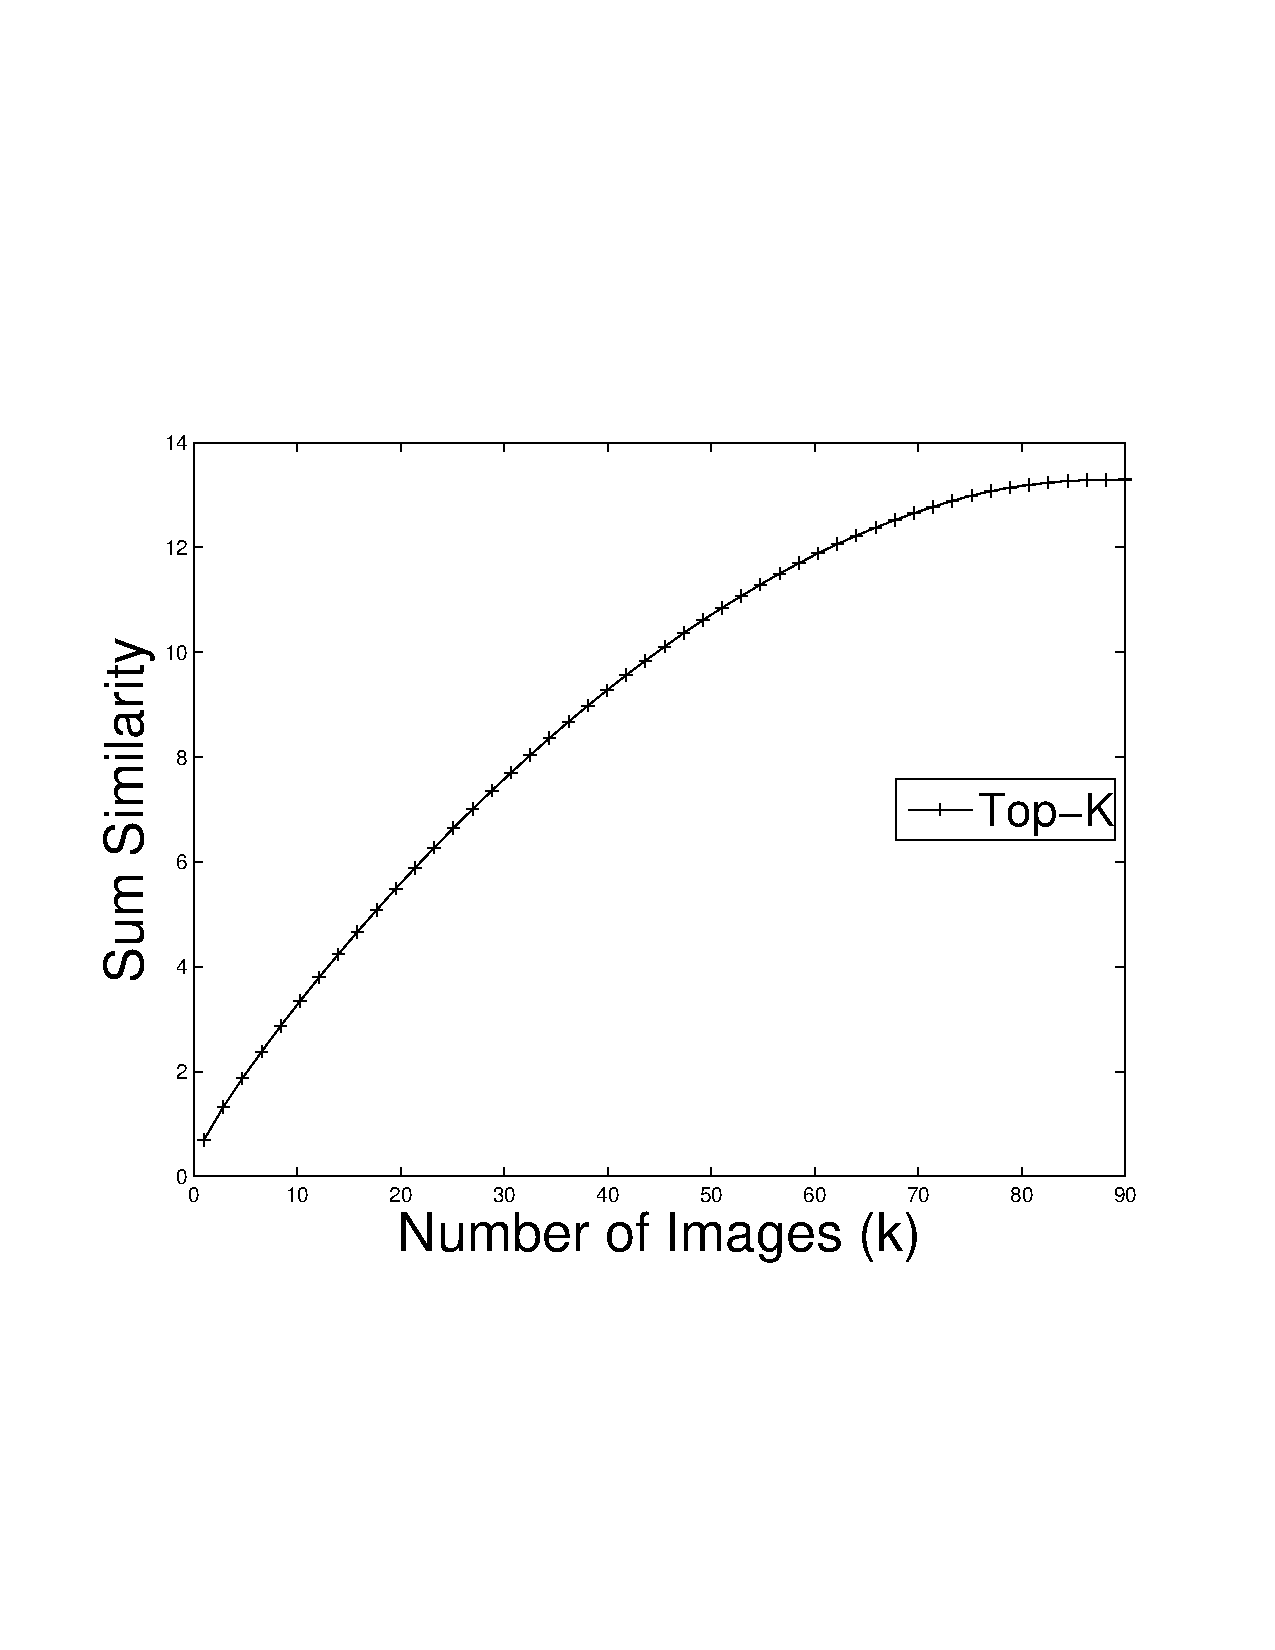
\includegraphics[clip=true, trim = 15mm 65mm 25mm 70mm, scale=0.23]{figures/USC_sumsim_topk.pdf}
        \label{fig:topkSumSim}
        }
    \subfigure[Top-K: Expected Sets Covered]{
        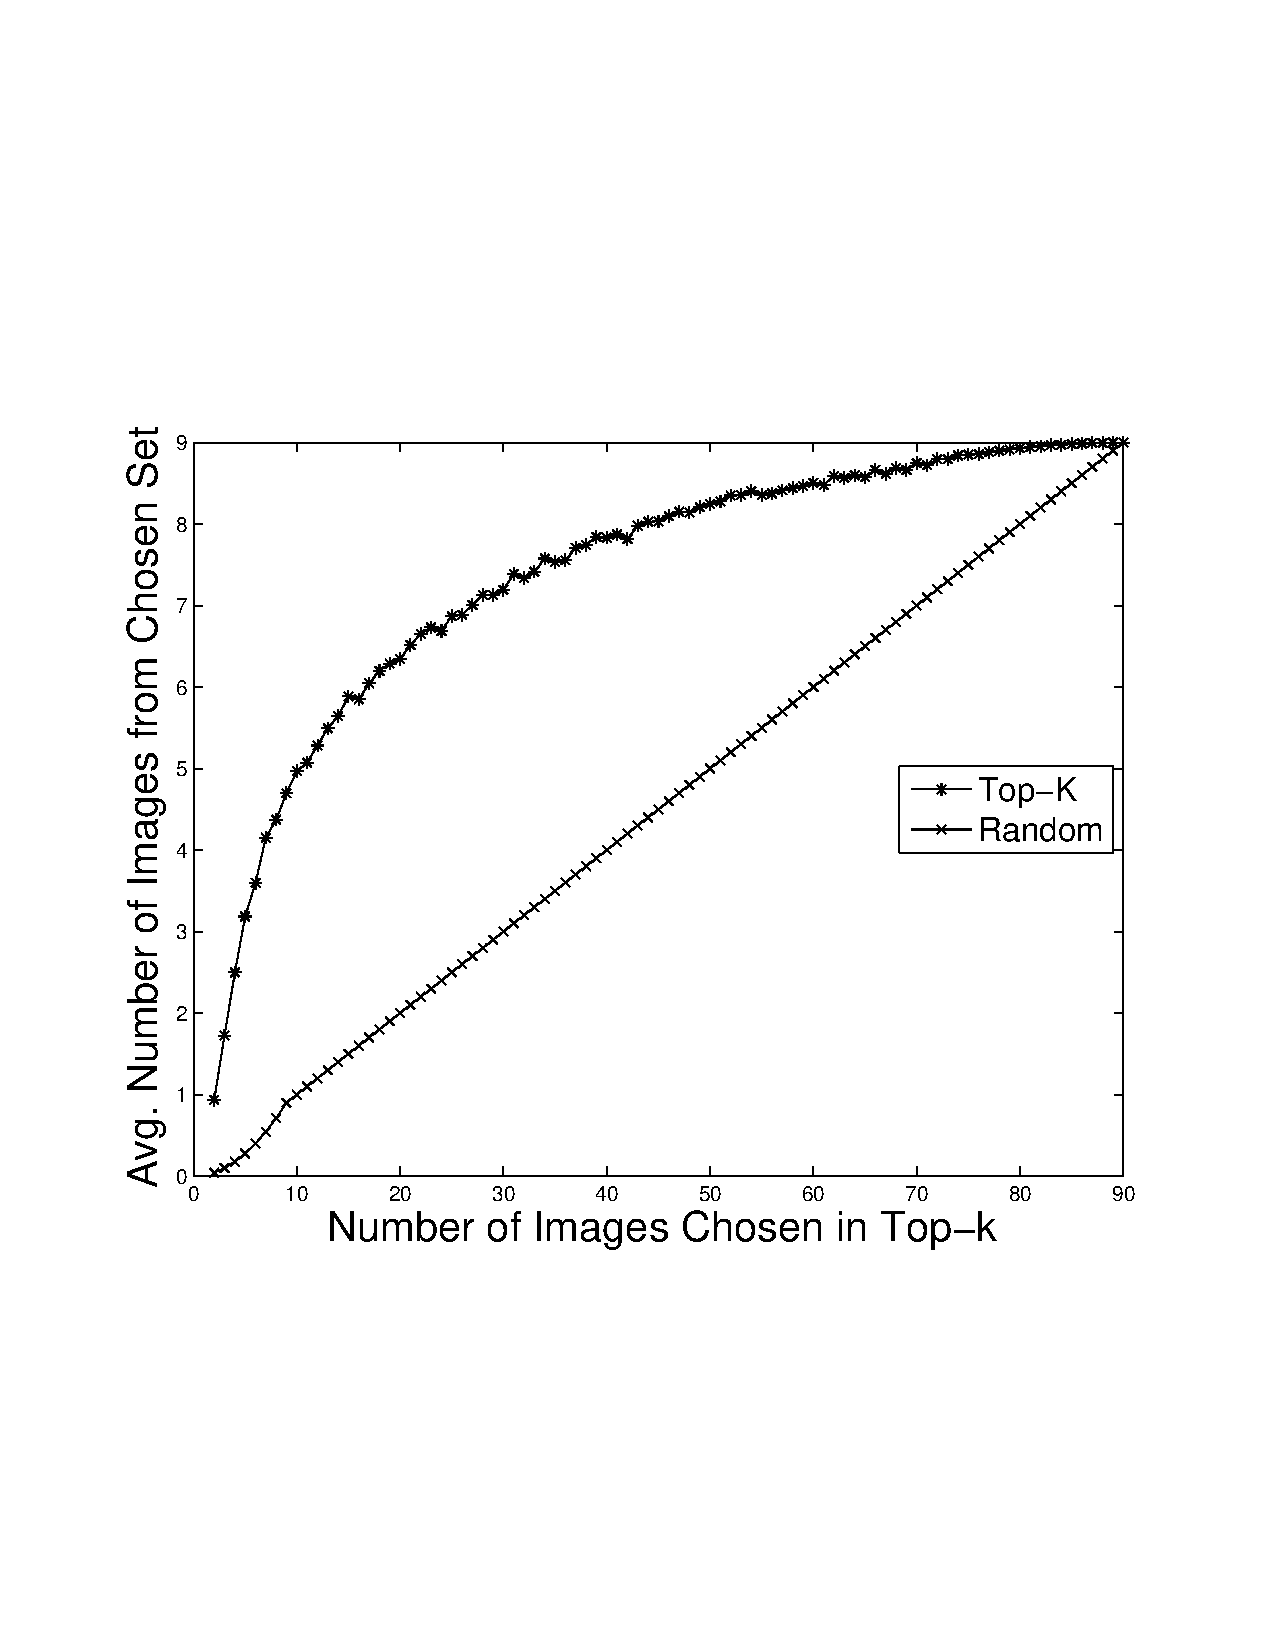
\includegraphics[clip=true, trim = 15mm 65mm 20mm 70mm, scale=0.23]{figures/topk/avg_num_matching.pdf}
        \label{fig:topkAvgNumSameSet}
        }
    \subfigure[Spanner: Sum Dissimilarity]{
        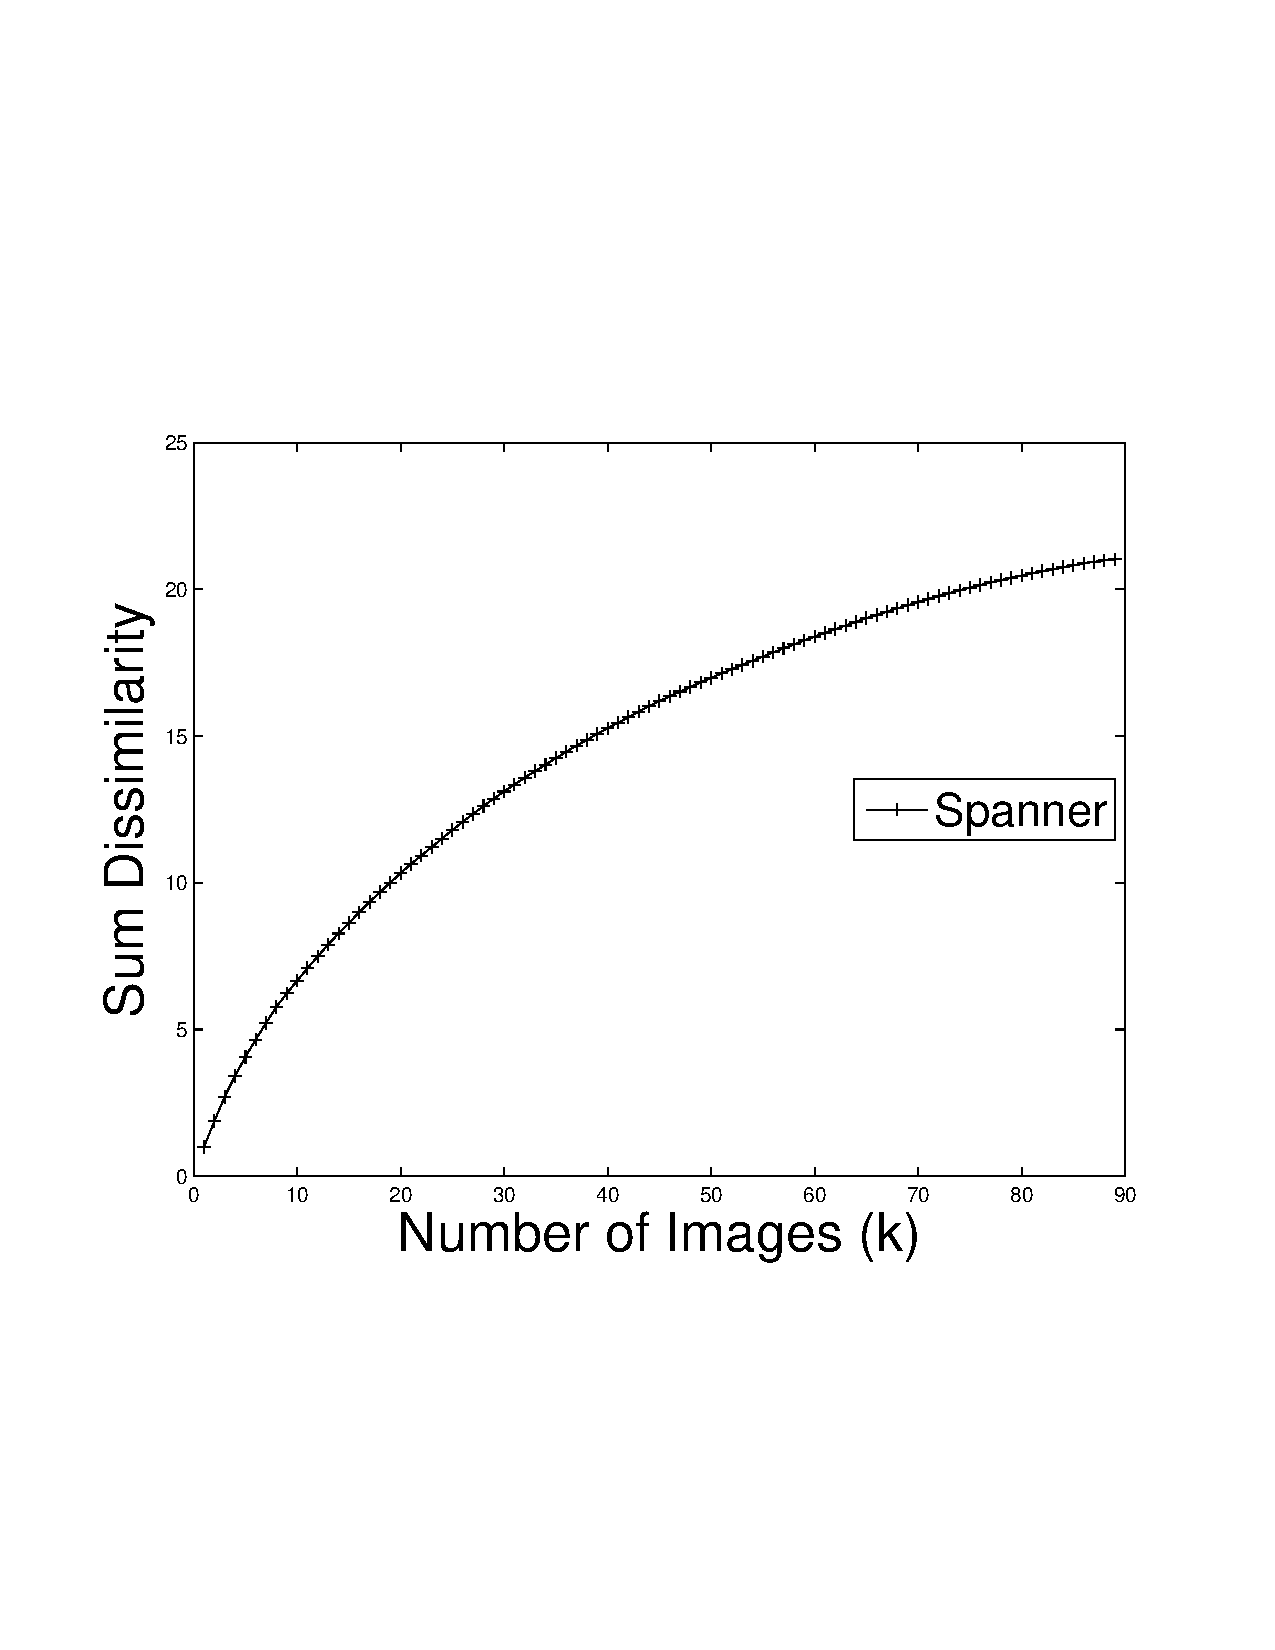
\includegraphics[clip=true, trim = 15mm 65mm 20mm 70mm, scale=0.23]{figures/spanner/spannerCumulativeDist.pdf}
        \label{fig:spanSumDissim}
        }
    \subfigure[Clustering: Prob. all Sets Covered]{
        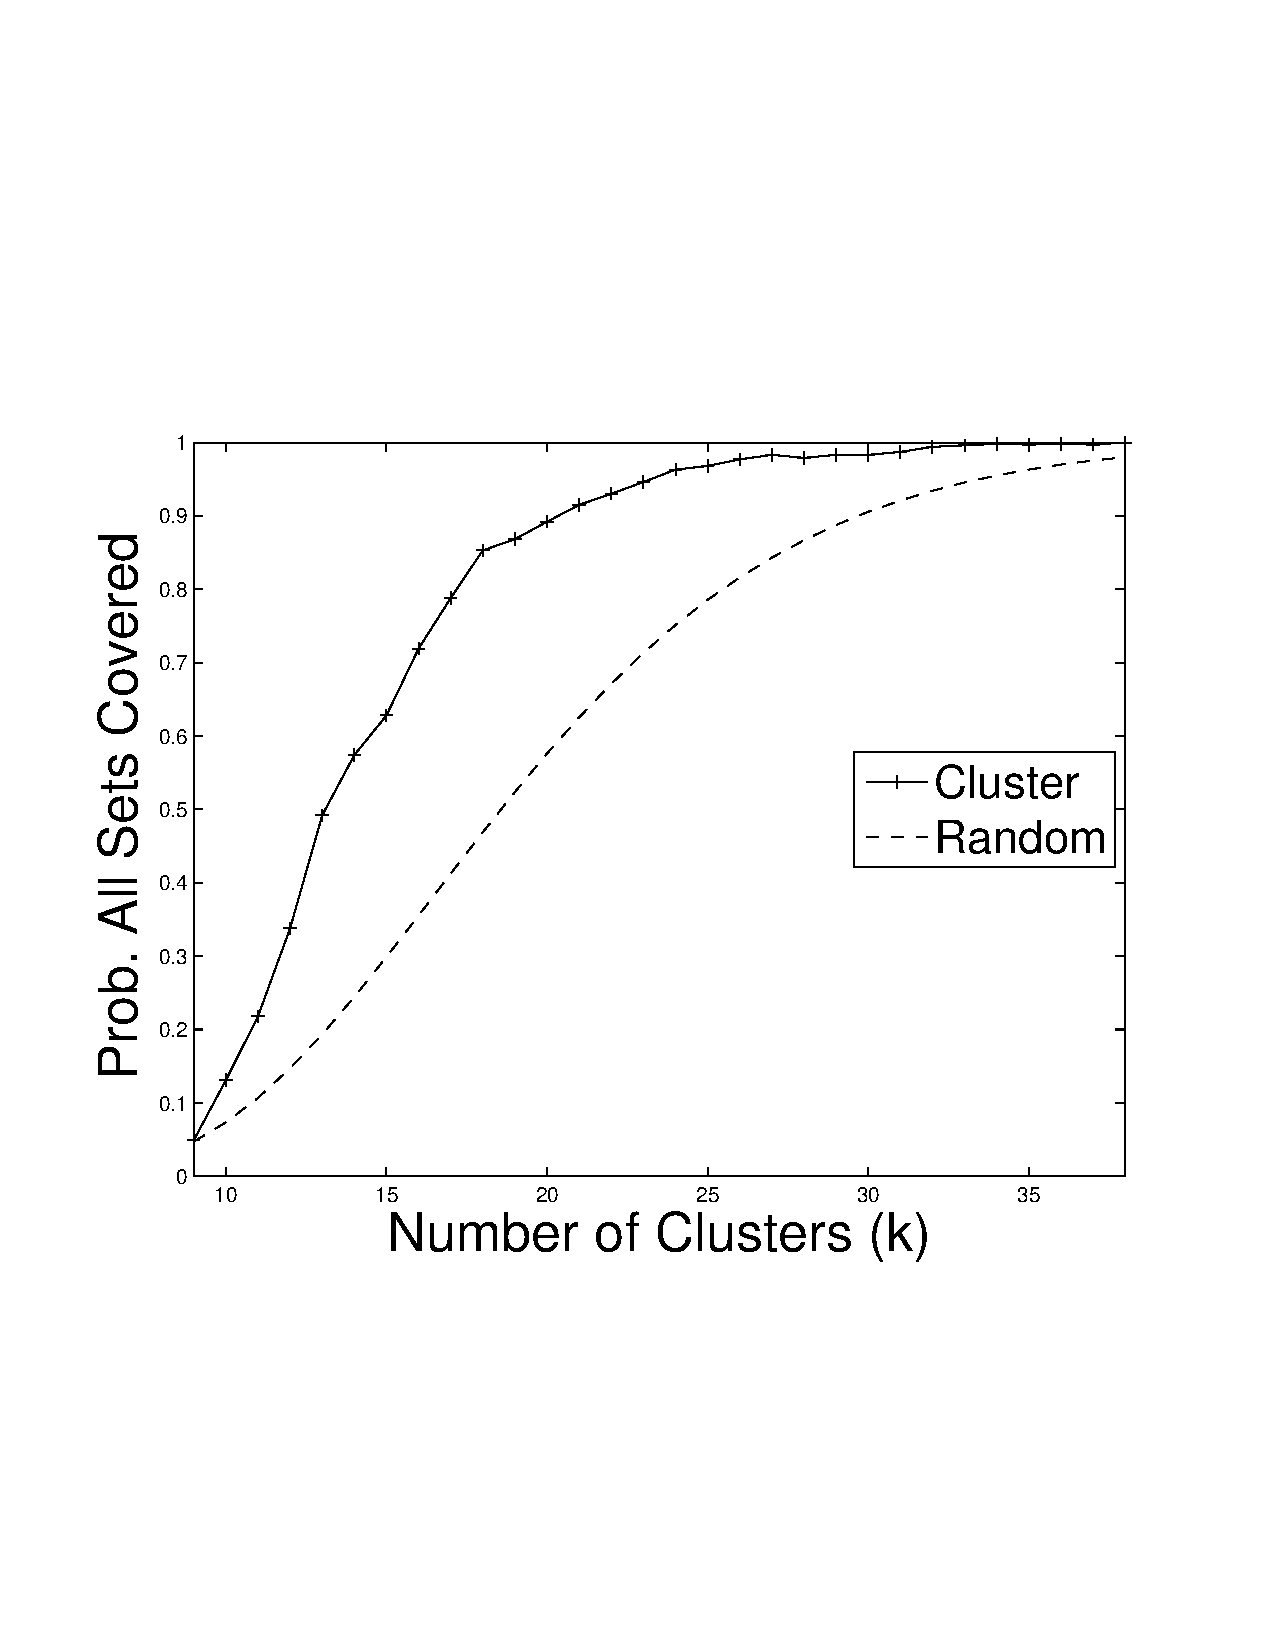
\includegraphics[clip=true, trim = 15mm 65mm 20mm 70mm, scale=0.23]{figures/cluster/perc_all_sets_covered_vary_k.pdf}
        \label{fig:clusterAvgNumSetsCov}
        }
        
        \vspace{-1mm}
   \caption{Completeness metrics for the three image selection algorithms. Each exhibits a diminishing return as more images are added.}
   \label{fig:completeness_exp_results}
   \vspace{-6mm}
\end{figure*}

QoI is a metric that can be defined for an application to give a more meaningful value to information by capturing attributes such as  timeliness, age/freshness, completeness, accuracy, precision, etc.  
For example, information that contributes to a decision-making process may only be useful if it arrives before the decision must be made, or it may have varying usefulness based on how similar or dissimilar it is to other data already collected.

The specific details of which attributes are considered and how they contribute to QoI is application-dependent.  The chosen QoI metrics are stored as a vector associated with a data item.  There are two ways to define QoI using that vector.  In one, a QoI function is defined that accepts the vector of metrics and provides a scalar value as an output like in  \cite{qoi_aware_mobile_apps,qoi_aware_trx_pol_time_vary_links} and many others.  In the second, as explained in \cite{qoi_aware_tactical_mil_nets}, a vector of minimum values for each QoI metric can be specified, and data can be evaluated based on whether it satisfies all of the QoI requirements or not.  We choose the latter method of determining QoI and focus on establishing the edges of QoI satisfiability for the vector of metrics, which defines the boundaries of maximum achievable QoI regions in the metric space.

We choose to use two QoI attributes, one that is time-based and one that is information-content-based.  The first attribute, whose importance has already been described, is timeliness, $T$, of data.  For the second attribute, we present a notion of \emph{completeness}, $C$, which we show can be defined multiple ways, depending on the context.  Together, a QoI requirement of $\mathbf{q} = \{C,T\}$ specifies a quantity of data that must be delivered as well as a deadline by which it must arrive to be useful.  While timeliness is not necessarily a new concept, completeness is less well defined.  Therefore, we identify three image selection algorithms, one that selects images based on similarity and two that select images based on diversity, and show how they can be evaluated with completeness.

\subsection{Image Selection Algorithms}

As a motivating example, we choose a network in which nodes store photographs that are to be exchanged or collected at one or more data sinks.  This example covers surveillance missions of military tactical networks or camera sensor networks.  Without adopting any one specific application, we present two query algorithms from \cite{mediascope}, one that helps return images similar to a target, and one that helps return a diverse set of images.  We also present ways to measure the completeness of each, providing a quantified value of a QoI metric.

Each of these queries require measuring the similarity or dissimilarity of two images.  To get a similarity measurement, we use the same choice as was shown to be effective in \cite{mediascope}.  This similarity is based on a technique called Color and Edge Directivity Descriptor (CEDD) \cite{2008cedd}, which uses qualities inherent to a photograph like lightness, contrast, and color.  The similarity between two images can then be given as a scalar by calculating the \emph{Tanimoto Similarity} \cite{tanimoto} between their CEDD vectors.  The dissimilarity value is simply defined as $1$ minus the similarity.

\subsubsection{Selecting Similar Images}

The first type of query we introduce occurs when a user already has one image of a particular area or object of interest and would like to obtain similar images to get a more complete view of that specific scene or object.  For example, if a user has a picture of an unknown suspicious person entering a building, but the person is not identifiable from that image, it would be useful to collect more images that are similar to that one with the possibility that another picture may have a better view of the person in question that can be used for identification or more context.  Called {\bf Top-K}, the query algorithm used for this application will choose the $k$ images with the most similarity with respect to the target image.  

Considering the goal of the Top-K query, we can evaluate the completeness of the result in one of two ways.  First, we can use the similarity of the images as a value representing each image's effectiveness in providing a more complete view of the target object or scene.  If we sum the similarity of all $k$ images returned by the algorithm, we get a representation of completeness, which we naturally call \emph{Sum Similarity}.  While this measure of completeness is abstract, it can be refined in an actual implementation through testing and evaluating.  This definition of completeness is useful, though, because it can be applied without any predetermined knowledge of the environment or pool of images.  

Often, though, we can partition the environment in which the network operates into a number, $n$, of distinct settings or areas.  In those cases, we can utilize a second method of quantifying completeness.  Assume that each image belongs to one of these $n$ sets, %$Q_i$, 
related to the setting it depicts.  Naturally, then, when executing a Top-K query, the goal is for the algorithm to return images from the same set as the target image.  Completeness can then be given by the fraction of images returned that are in the same set as the target image.

\subsubsection{Selecting Diverse Images}

In contrast, given the set of all photographs available in the network, we might want to return the set of $k$ images that exhibits the most diversity, ideally providing a user with a good sampling, or \emph{complete view}, of available images.  For instance, such a result would be quite useful in a surveillance mission.  We present two query algorithms that can be used to achieve this goal.

One query that provides diverse images is known as the {\bf Spanner} of the set of known photographs.  For the Spanner algorithm, we employ a greedy algorithm similar to that in \cite{mediascope} to simplify implementation and to define a \emph{Sum Dissimilarity} metric.  Here, the algorithm first chooses the two images with the greatest dissimilarity between them from all available images.  Then, each successive image is chosen to be the one with the greatest minimum distance between it and all images already chosen, until $k$ images are selected.  This minimum distance between the image being selected and the images in the collected set is the value added to the running cumulative completeness metric of \emph{Sum Dissimilarity}.  Since the Spanner algorithm's goal is to provide images at the edges of the available feature space, the Sum Dissimilarity represents a measure of its completeness because a higher level of dissimilarity is providing a more complete view of the feature space.

The other query that can achieve a complete view over all images is {\bf Clustering}.  In the Clustering algorithm, all images are separated into a $k$ clusters based on their pairwise distances using any version of a k-means clustering algorithm, where $k$ is given by the user.  Then, the most central image from each cluster is returned.  
Here, assuming that the photographs of the same settings or objects of interest exhibit similar characteristics, Clustering should provide a complete view of the network's environment.

Both Spanner and Clustering algorithms can also be evaluated using the model in which the environment is split into $n$ sets.  With this model, we can define completeness as either the number of sets represented by at least one of the $k$ images returned or the probability of all $n$ sets being represented by at least one image when $k$ are returned.  Here, though, we only show results for the second definition.

\subsubsection{Experimental Results}

%%Top-K Sum Similarity
%\begin{figure} 
%\centering
%    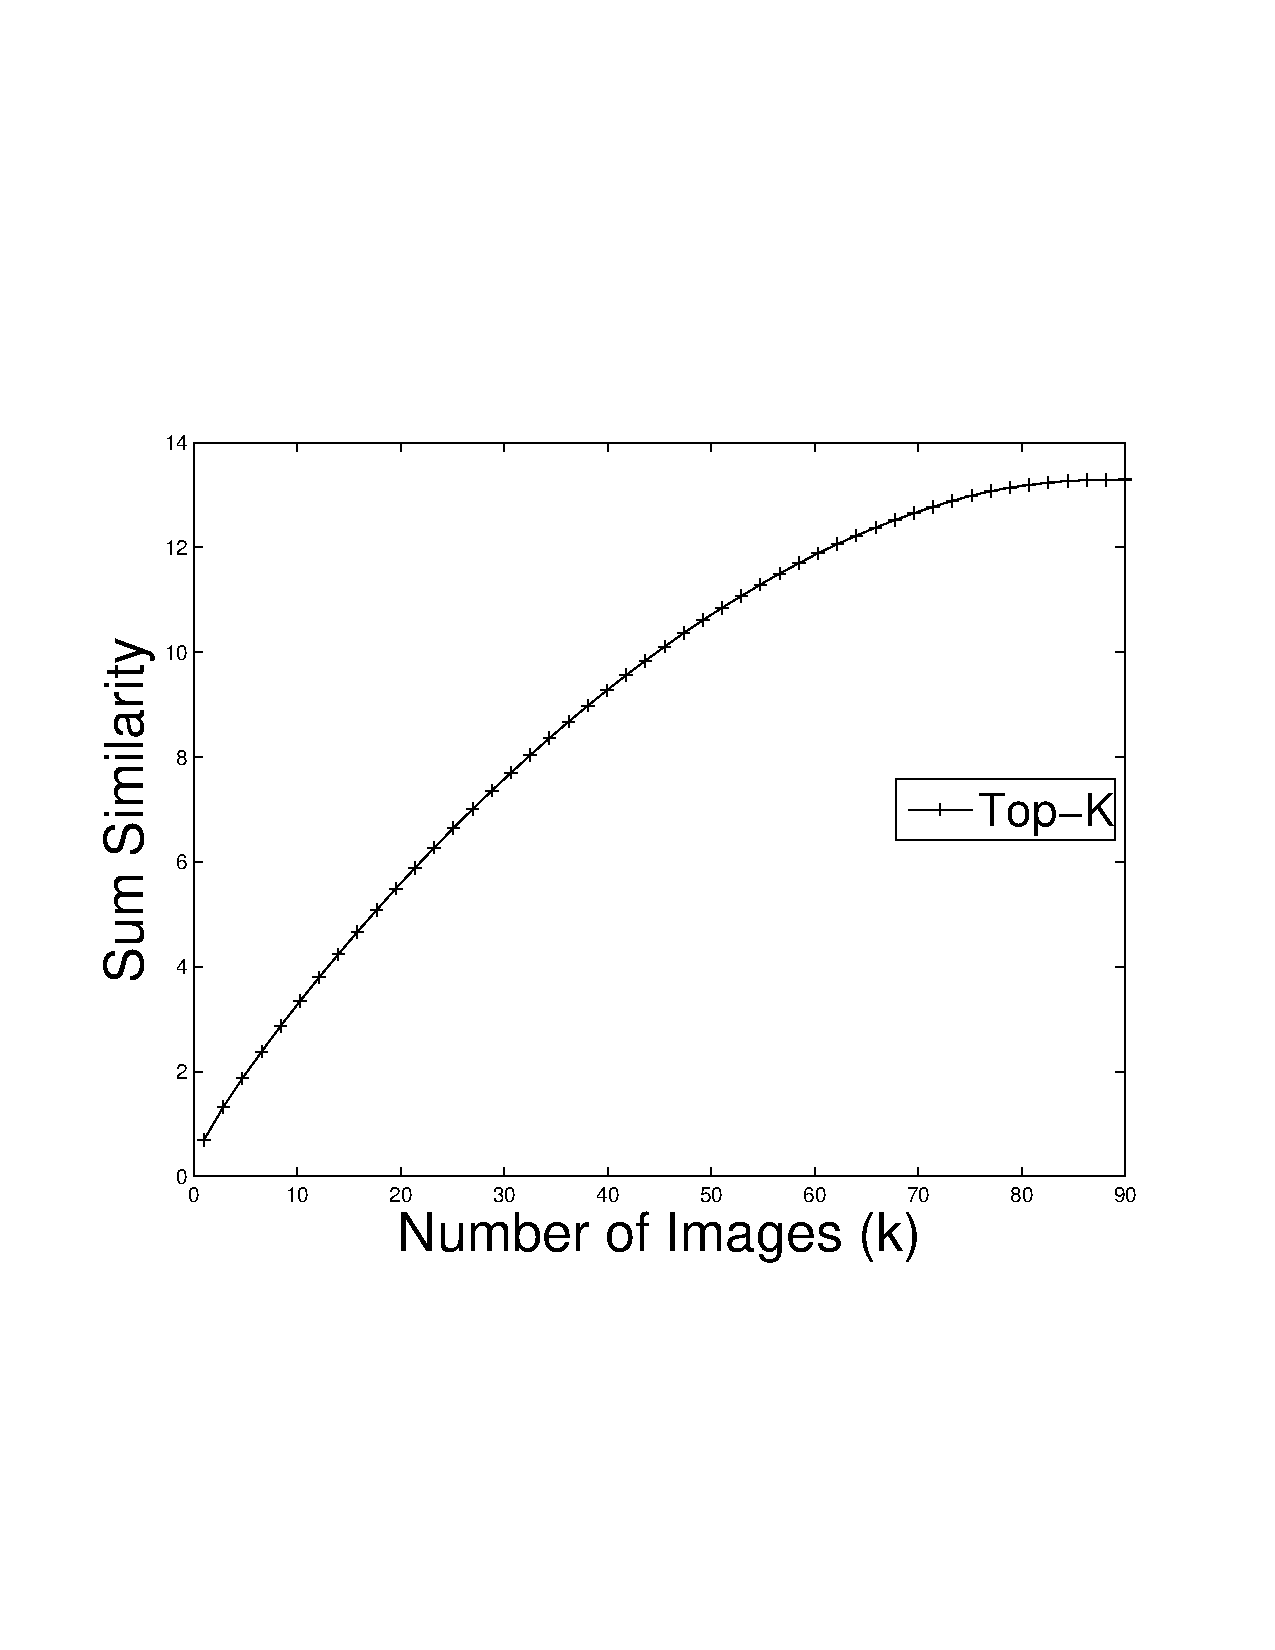
\includegraphics[clip=true, trim = 20mm 65mm 25mm 70mm, scale=0.35]{figures/USC_sumsim_topk.pdf}
%    \vspace{-4mm}
%    \label{fig:topkSumSim}
%    \vspace{-3mm}
%\end{figure}
%
%% Top-K Average Number from Same Set Returned
%\begin{figure} 
%\centering
%    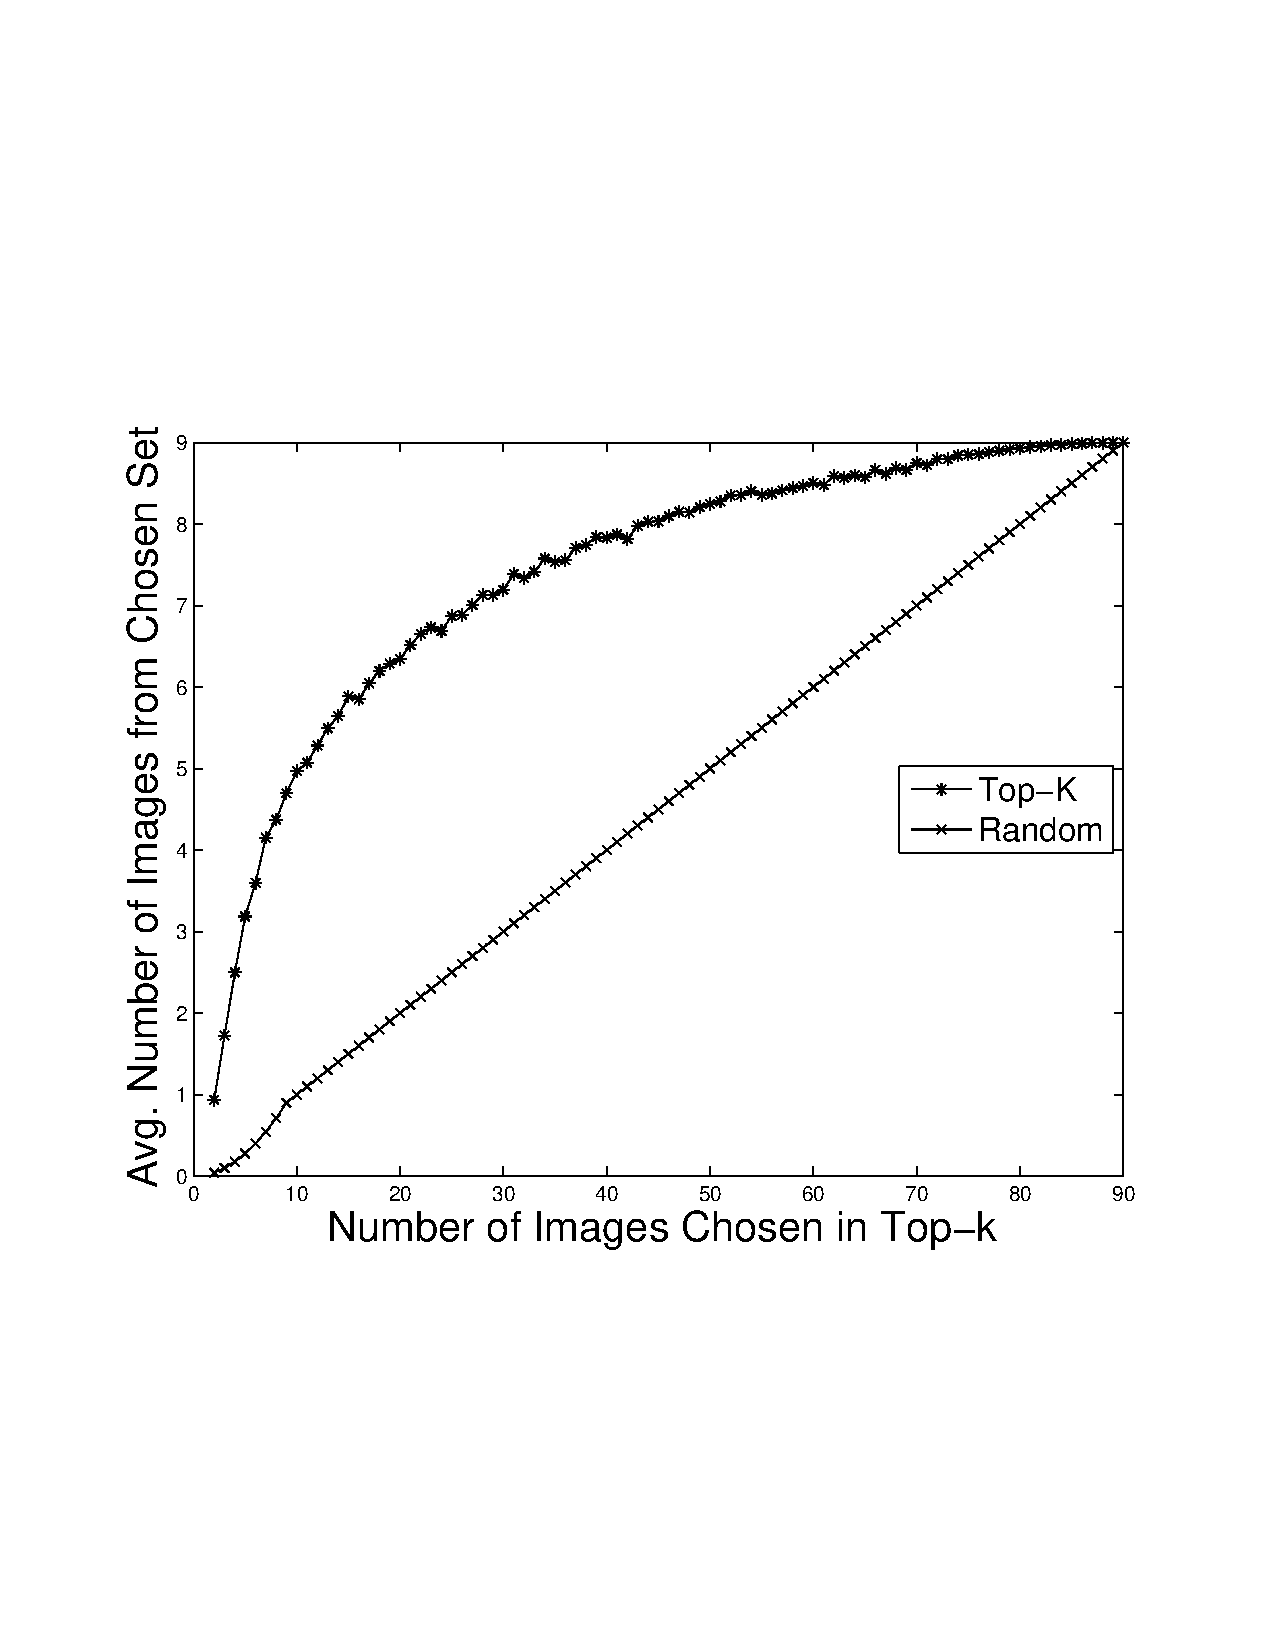
\includegraphics[clip=true, trim = 15mm 65mm 20mm 70mm, scale=0.35]{figures/topk/avg_num_matching.pdf}
%    \vspace{-3mm}
%    \caption{Top-K algorithm performs returns more images from target set than random, but also exhibits diminishing returns as $k$ increases.}
%    \label{fig:topkAvgNumSameSet}
%    \vspace{-6mm}
%\end{figure}

To provide example values of these completeness metric definitions, experiments applying each query algorithm were run on a set of pictures taken at $n = 9$ different settings around the Penn State campus.  Each of these $9$ settings is of a pictorially different area, e.g. a particular building, a downtown street, or a lawn setting, and over $20$ images of each was taken.  Then, for individual trials, $10$ images from each set were randomly selected to create an image pool of $90$ pictures.  The three algorithms were run over these $90$ images, with the target image being randomly selected in the case of Top-K.  Results for each of the different completeness metrics were averaged over $1,000$ trials are shown in Figures \ref{fig:topkSumSim} to \ref{fig:clusterAvgNumSetsCov}.

Figure \ref{fig:topkSumSim} shows the average sum similarity of images returned by the Top-K algorithm.  Figure \ref{fig:topkAvgNumSameSet} provides the second definition of completeness for the Top-K algorithm, the number of images matching the set that the target image was randomly chosen from.  
Completeness results when dissimilarity is the objective are shown in Figures \ref{fig:spanSumDissim} and \ref{fig:clusterAvgNumSetsCov}.  Specifically, Figure \ref{fig:spanSumDissim} depicts the average Sum Dissimilarity returned by the Spanner algorithm, and 
Figure \ref{fig:clusterAvgNumSetsCov} represents the empirical probability of all $9$ sets being represented in the $k$ returned images.   For reference, we also include expected values for the metrics in Figures \ref{fig:topkAvgNumSameSet} and \ref{fig:clusterAvgNumSetsCov} if the images were selected from the entire image pool at random, i.e., without regard for image similarity or dissimilarity.  

All of these figures exhibit the diminishing returns of completeness as more images are collected.  This effect is important because it visually shows how QoI differs from throughput.  As seen in these graphs, transmission of successive images does not result in a linear gain in completeness.  For example, in Figure \ref{fig:topkAvgNumSameSet}, it is evident that a value of only $k \approx 10$ is needed to collect $5$ images matching the target content, while collecting an additional $2$ from the same set usually requires collecting over twice that number of pictures.  

As a second example, Figure \ref{fig:clusterAvgNumSetsCov} shows that jumping from $k=10$ to $k=20$, the likelihood of capturing at least one image of every setting grows substantially from just over $10\%$ to approximately $90\%$.  To approach probabilities close to gaining that final $10\%$, however, requires a jump to $k\approx30$.  

%%Spanner Sum Dissimilarity
%\begin{figure} 
%\begin{centering}
%    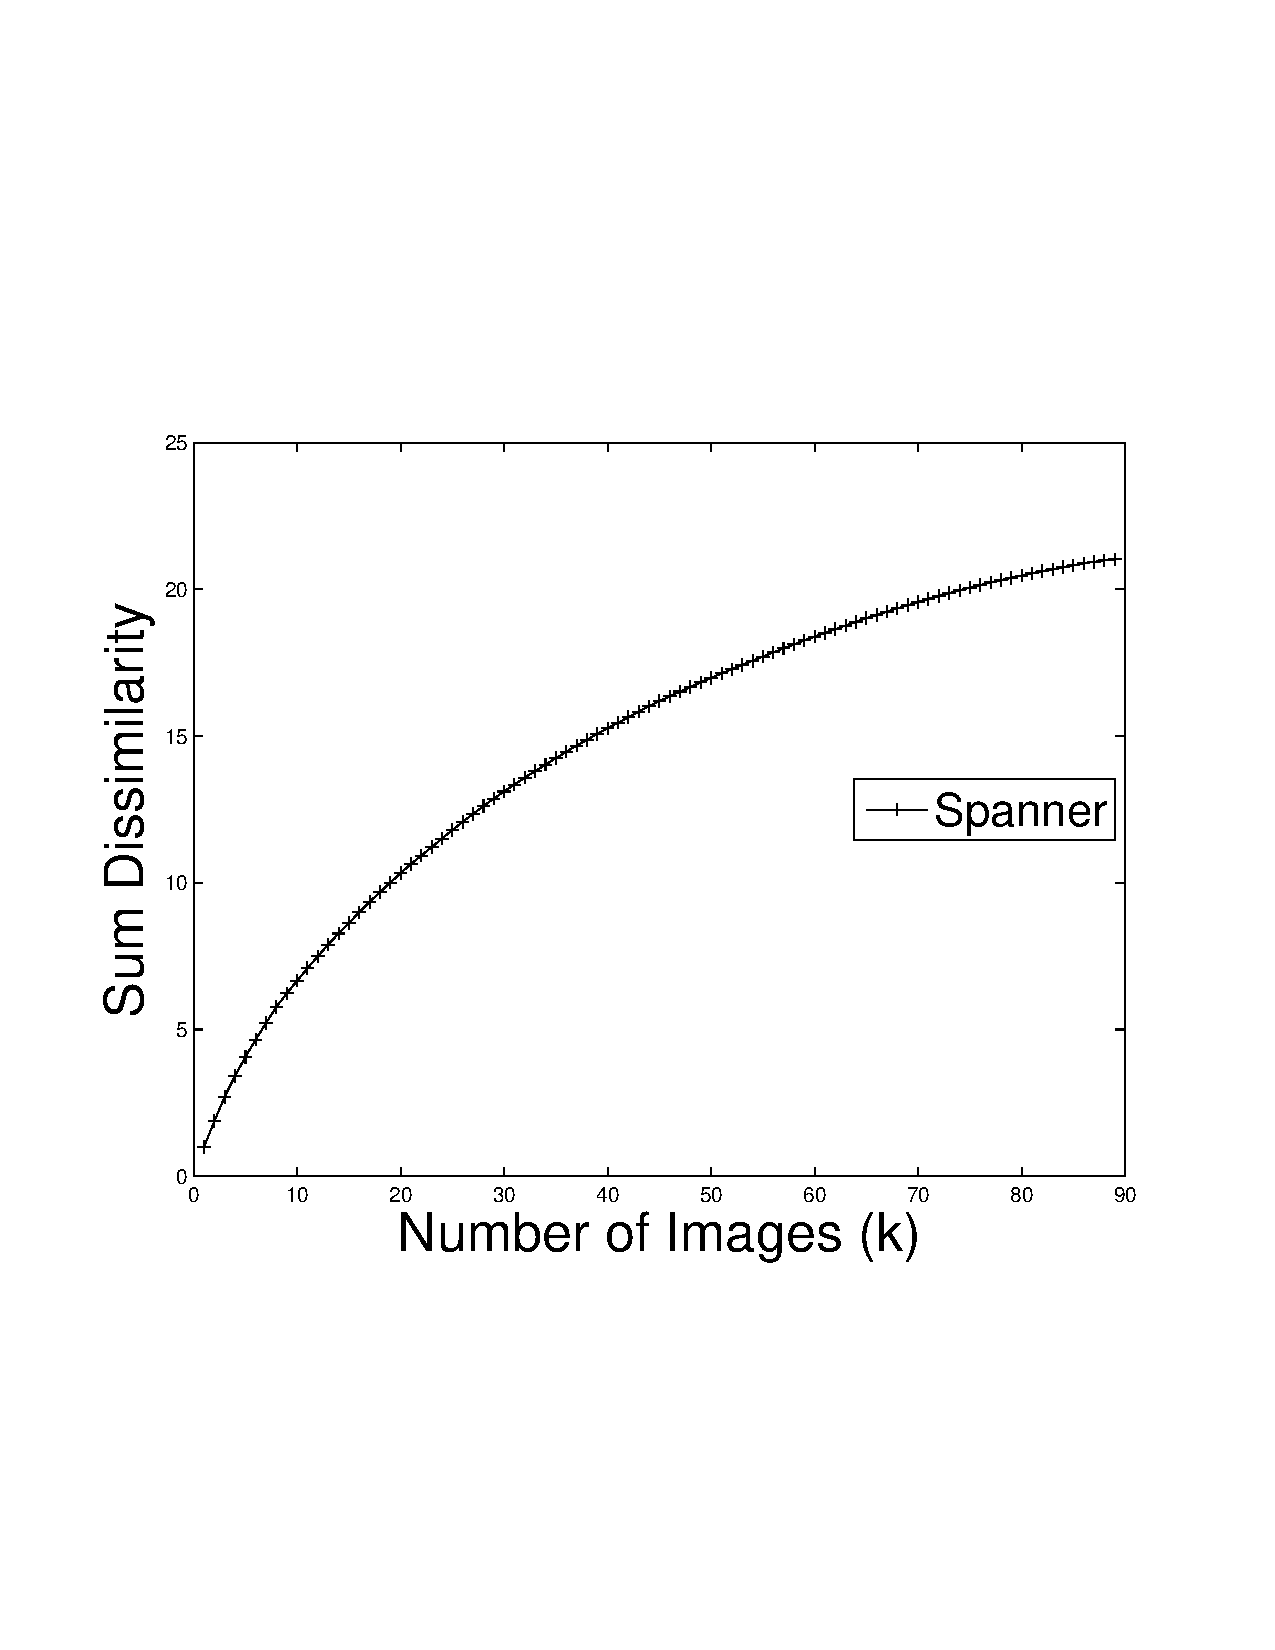
\includegraphics[clip=true, trim = 15mm 65mm 20mm 70mm, scale=0.35]{figures/spanner/spannerCumulativeDist.pdf}
%    \vspace{-3mm}
%    \caption{Diminishing returns on Sum Dissimilarity exhibited by the Spanner algorithm as more images are retrieved.}
%    \label{fig:spanSumDissim}
%    \vspace{-3mm}
%\end{centering}
%\end{figure}
%
%% Cluster Percentage All Sets Covered
%\begin{figure} 
%\begin{centering}
%    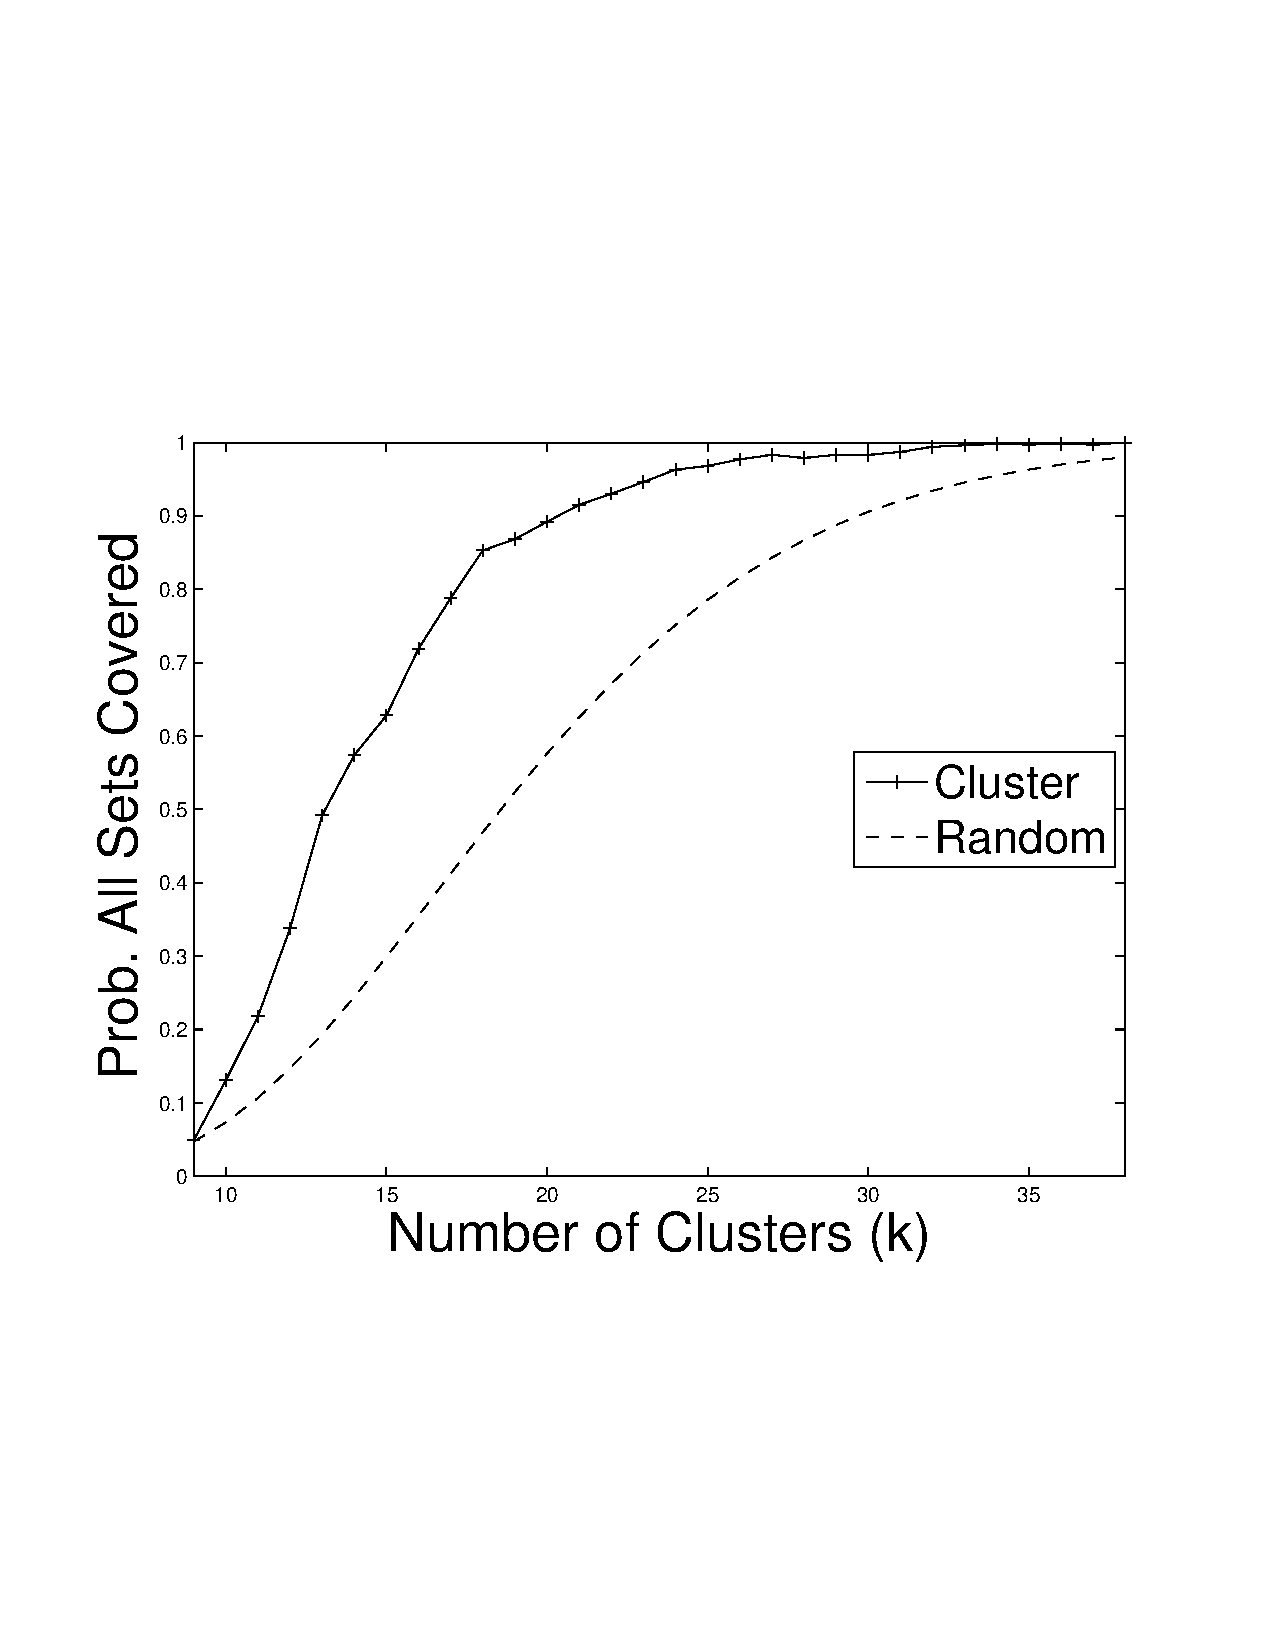
\includegraphics[clip=true, trim = 15mm 65mm 20mm 70mm, scale=0.35]{figures/cluster/perc_all_sets_covered_vary_k.pdf}
%    \vspace{-3mm}
%    \caption{Empirical probability of obtaining at least one image from every set as $k$ is increased with the Clustering algorithm.  A highly non-linear, diminishing returns effect is seen.}
%    \label{fig:clusterAvgNumSetsCov}
%    \vspace{-7mm}
%\end{centering}
%\end{figure}

The relationship between the number of images and completeness in each of these graphs also shows that obtaining a certain value of QoI or completeness requires a different number of images depending on the set available and their similarities.  We can denote the number of images required to achieve a level of completeness, $C$, as $k_{req} = Q(C)$.  This relationship will be useful later in determining capacity and scalability limits.

\subsection{Further Discussion of QoI}
We have defined and provided examples for a number of ways that completeness can be defined and used to obtain a concrete data requirement from a contextual QoI requirement.  Throughout the rest of the paper, we mainly use sum similarity as the completeness metric, but any of the definitions of completeness used here, or any other QoI requirement that can be translated into a data requirement, for that matter, can be used in the following formulation in Section \ref{sec:qoi_scalability}.

Also, note that QoI and its usage in understanding networks is not exclusive to these metrics and applications.  On the contrary, the model used in the capacity and scalability analysis of Section \ref{sec:qoi_scalability} is meant to be an in-depth example of this concept.  Modifications to account for different data size requirements should be quite straightforward, and extensions to other time-based metrics should be possible with careful extensions to the framework.

Finally, while metadata associated with photographs may be useful in obtaining similar goals to those given in this section, relying on such information is problematic because metadata is not guaranteed to be available, and it is not as universally applicable as content-based retrieval.  For example, tags describing the image contents would require users to participate by entering this information, which is a time-consuming and unreliable step that users are likely to ignore.  Location and time stamps may be automatically applied by the device allowing an application to filter images accordingly, but these tags often do not account for factors such as the direction of the camera or obstructed views.  Content-based processing of these images, though, can be applied to any set of images.





\section{QoI Scalability}
\label{sec:qoi_scalability}

\begin{figure}
\centering
    \subfigure[$TF = 2$, $CF = 3$, $DF = 1$]{
        \includegraphics[scale=0.28, clip=true, trim=5mm 0mm 5mm 0mm, valign=t]{delay_expl_fig_a.pdf}
        \label{fig:delay_expl_fig_3}
        }
    \subfigure[$TF = 2$, $CF = 3$, $DF = 2$]{
        \includegraphics[scale=0.28, valign=t]{delay_expl_fig_b.pdf}
        \label{fig:delay_expl_fig_4}
        }

   \caption{Example of line network using TDMA highlighting source of delays. (Node labels are TDMA slot assignments.)}
   \label{fig:both_delay_figures}
   \vspace{-5mm}
\end{figure}

Given the nonlinear returns of completeness and importance of timeliness outlined in the previous section, we contend that simply establishing the highest average supportable rate should not be the only goal of a QoI-aware network.  With this knowledge, we set the goal of determining the capacity of a network (and relatedly, the scalability achievable) with respect to {\em QoI requirements}, instead of the maximum throughput.  

\subsection{QoI Satisfiability Framework}
In order to establish the framework, we examine an arbitrary flow, $F_1$, in the network that has a QoI requirement of $\mathbf{q} = \{C, T\}$, where $C$ is the minimum required completeness metric of choice, such as sum similarity as explained above, and $T$ is the required timeliness.  This flow will have a data size requirement, which is given by a chosen QoI function $Q(C)$ like those discussed in Section \ref{sec:qoi_model}.  Using the example applications from \ref{sec:qoi_model}, for example, $Q(C)$ can return the number of images, $k_{req}$, required to achieve the requested completeness $C$ according to established relations like those in Section \ref{sec:qoi_model}.  Assuming each image has an average size of $I_S$, then we can also use $B$ to describe the total number of bits required by the flow, $B=k_{req}*I_S$.  To match realistic network implications, we assume this data will be transmitted in a series of packets with size $P_S$ bits each.  The number of packets per flow, then, is simply $P_N = \lceil B/P_S \rceil$.  We assume that each node in the network can transmit at $W$ bits per second when it is allocated media access.

Our goal is to establish the limits at which this arbitrary flow on average can no longer be completed with the QoI requirements satisfied.  We build and explain our model for achieving this goal by working through an example TDMA line network, a portion of which is shown in Figures \ref{fig:delay_expl_fig_3} and \ref{fig:delay_expl_fig_4} (We discuss addressing non-TDMA networks in Section \ref{sec:discussion}).  In this network, we assume a simple 3-slot TDMA scheme, which allows each node equal time access to the medium and removes any potential interference or hidden terminal issues.  Each node in the figure is labeled with its allocated slot.  For simplicity, we will assume that one slot is appropriately sized to transmit a single packet, i.e., $T_{slot} = P_S/W$ and that packets use static routes calculated beforehand such that the overhead is not a consideration here.

Now, two factors, $D_1$ and $D_2$, contribute to the total delay of completing $F_1$.  The first contributor, $D_1$, is the end to end delay incurred by sending the $B$ bits across the entire path.  To quantify this delay, we must consider several factors beyond just the available bandwidth and number of packets.  First, each node can only utilize its allotted channel time, creating a Channel Factor of $CF = N_{frame}/N_{i}$, where $N_{i}$ is the number of slots allocated to node $i$ and $N_{frame}$ is the total number of slots in each frame.  In this case, $N_{i} = 1, \forall i$ and $N_{frame} = 3$.  The second factor to consider for $D_1$ is the fraction of allocated slots that are utilized by the node to serve flows other than $F_1$ that are either originating in or being routed through nodes on the path of flow $F_1$.  We call the total number of flows competing at node $i$ the Traffic Factor, $TF_i$, of that node.  For any flow, the maximum contributor to delay is the node along the path with the maximum $TF_i$, which we will just call $TF$ here.  Incorporating these considerations into a calculation for $D_1$, we achieve the following expression


\begin{equation}
	D_1 = T_{slot} \cdot P_N \cdot CF \cdot TF
\end{equation}
%\begin{figure}
%\begin{centering}
%    \includegraphics[scale=0.33]{figures/delay_limit_expl/delay_expl_fig_a.pdf}
%    \caption{Example of line network using TDMA highlighting source of delays, $D_1$ and $D_2$.  Here, $TF = 2$, $CF = 3$, and $DF = 1$. }
%    \label{fig:delay_expl_fig_3}
%    \vspace{-3mm}
%\end{centering}
%\end{figure}

Figure \ref{fig:delay_expl_fig_3} depicts the delay of $D_1$ in a simple case of only two flows, $F_1$ and $F_2$, being present, in which case $TF = 2$.  In this example we use flows that consist of only $2$ ($F_{i-j}$ is packet $j$ in flow $i$) packets to portray the delay.  In most real applications, $P_N$ will be much larger, making $D_1$ a good approximation of this delay component.

%\begin{figure}
%\begin{centering}
%    \includegraphics[scale=0.35]{figures/delay_limit_expl/delay_expl_fig_b.pdf}
%    \caption{In the opposite direction, $DF = 2$. ($TF$ and $CF$ are unchanged here.)}
%    \label{fig:delay_expl_fig_4}
%\vspace{-5mm}
%\end{centering}
%\end{figure}

The second delay that exists is due to multi-hop propagation of packets.  This delay is simply the time for a single packet to traverse the path length.  Note that this delay is not necessarily just the path length multiplied by $T_{slot}$, because of possible queuing delays and/or ordering constraints.  We show here how ordering constraints impact this TDMA network.  A node cannot forward a packet from the flow until it receives that packet from the previous hop.  In our line network example, when the direction of the flow matches the nodes' schedule of slots $1-2-3-1-2-3$, as in Figure \ref{fig:delay_expl_fig_3}, each successive node receives a packet on the time slot before it is scheduled, resulting in no extra delay.  For a flow in the opposite direction, though, where nodes are scheduled $3-2-1-3-2-1$, as in Figure \ref{fig:delay_expl_fig_4}, the first slot $1$ is not utilized, because the first node scheduled in time slot $1$ has not yet received a packet in the flow.  Every other slot is wasted, on average, for the initialization of the flow, resulting in approximately twice the delay.  We will use a term that we call the \emph{Delay Factor}, or $DF$, to account for this effect where it exists.

The multi-hop propagation delay, then, is modeled by

\begin{equation}
	D_2 = T_{slot} \cdot DF \cdot (PL - 1)
\end{equation}
where $PL$ is the average path length.

We note several points about this delay factor.  First, in a loaded network, the nodes can and will serve other flows while awaiting the arrival of packets in this flow of focus.  That utilized bandwidth does not, however, preclude this $DF$ impact on delay for the flow of interest, $F_1$.  Any node cannot serve $F_1$ until a packet from that flow has been received.  Second, this delay is only accounted for once per flow because all other packets are pipelined.  All other packets' delay is captured by the end to end delay, $D_1$.  This effect is best illustrated by examining the difference between $D_2$ in Figures \ref{fig:delay_expl_fig_3} and \ref{fig:delay_expl_fig_4}.  Here, we see the multi-hop propagation requires twice the number of slots because every other slot is unused in $F_1$'s propagation.  
%Note that these unused slots may be used by the nodes to transmit packets from a different flow, so the bandwidth may be utilized, but since it cannot be used for flow $F_1$, the delay for this flow is still impacted by $DF$.

To calculate a $DF$ for an entire network, we can calculate a $DF$ for each possible sample path and find the average of these values.  For example, in the case of the line network with a $3$-slot schedule, $DF = 1$ in the direction for Figure \ref{fig:delay_expl_fig_3} and $DF = 2$ in the opposite direction shown in Figure \ref{fig:delay_expl_fig_4}, so the average $DF$ used to approximate average delay in the network is $DF_{line-avg}=1.5$.  

By combining the two components of delay, we can give a relation for a network that will successfully achieve an average flow's data and timeliness requirements:

\vspace{-2mm}
\begin{equation*}
	D_1 + D_2 \leq T 
\end{equation*}
\begin{equation*}
	T_{slot} \cdot P_N \cdot CF \cdot TF + T_{slot} \cdot DF \cdot (PL-1) \leq T
\end{equation*}

Recalling that the time of a slot is determined by the size of a packet, $P_S$, and available channel rate, $W$, in the relation $T_{slot} = P_S/W$, we can substitute to get
\begin{equation*}
	\frac{P_S}{W} \cdot P_N \cdot CF \cdot TF + \frac{P_S}{W} \cdot DF \cdot (PL-1) \leq T
\end{equation*}
Finally, substituting the total number of bits required for a flow $P_S \cdot P_N =  k_{req} \cdot I_S$ (where $k_{req}$ is given by a function of required QoI), and rearranging this inequality, we can obtain a cleaner view of each parameter's impact on network limits:

\vspace{-2mm}
\begin{equation}
	W \cdot T - k_{req} \cdot I_S \cdot CF \cdot TF - P_S \cdot DF \cdot (PL-1) \geq 0	
	\label{eq:general_scal}
\end{equation}

Every network will have its own set of parameters that can be substituted into this general formula, providing a tool to approximate limitations and sensitivity to changes in specific parameters.  To show this usefulness concretely, we provide derived values for a TDMA-based wireless network with several basic topologies.


\begin{figure*}[]
\centering
    \subfigure[Clique Network, $I_S = 9 MB$]{
        \includegraphics[scale=0.29, clip=true, trim=15mm 65mm 20mm 65mm]{clique_uni_2d.pdf}
        \label{fig:scal_vs_qoi_clique}
        }
    \subfigure[Line Network, $I_S = 12 MB$]{
        \includegraphics[scale=0.29, clip=true, trim=15mm 65mm 20mm 65mm]{line_uni_2d_mhop_2.pdf}
        \label{fig:scal_vs_qoi_line}
        }
    \subfigure[Grid Network, $I_S = 48 MB$]{
        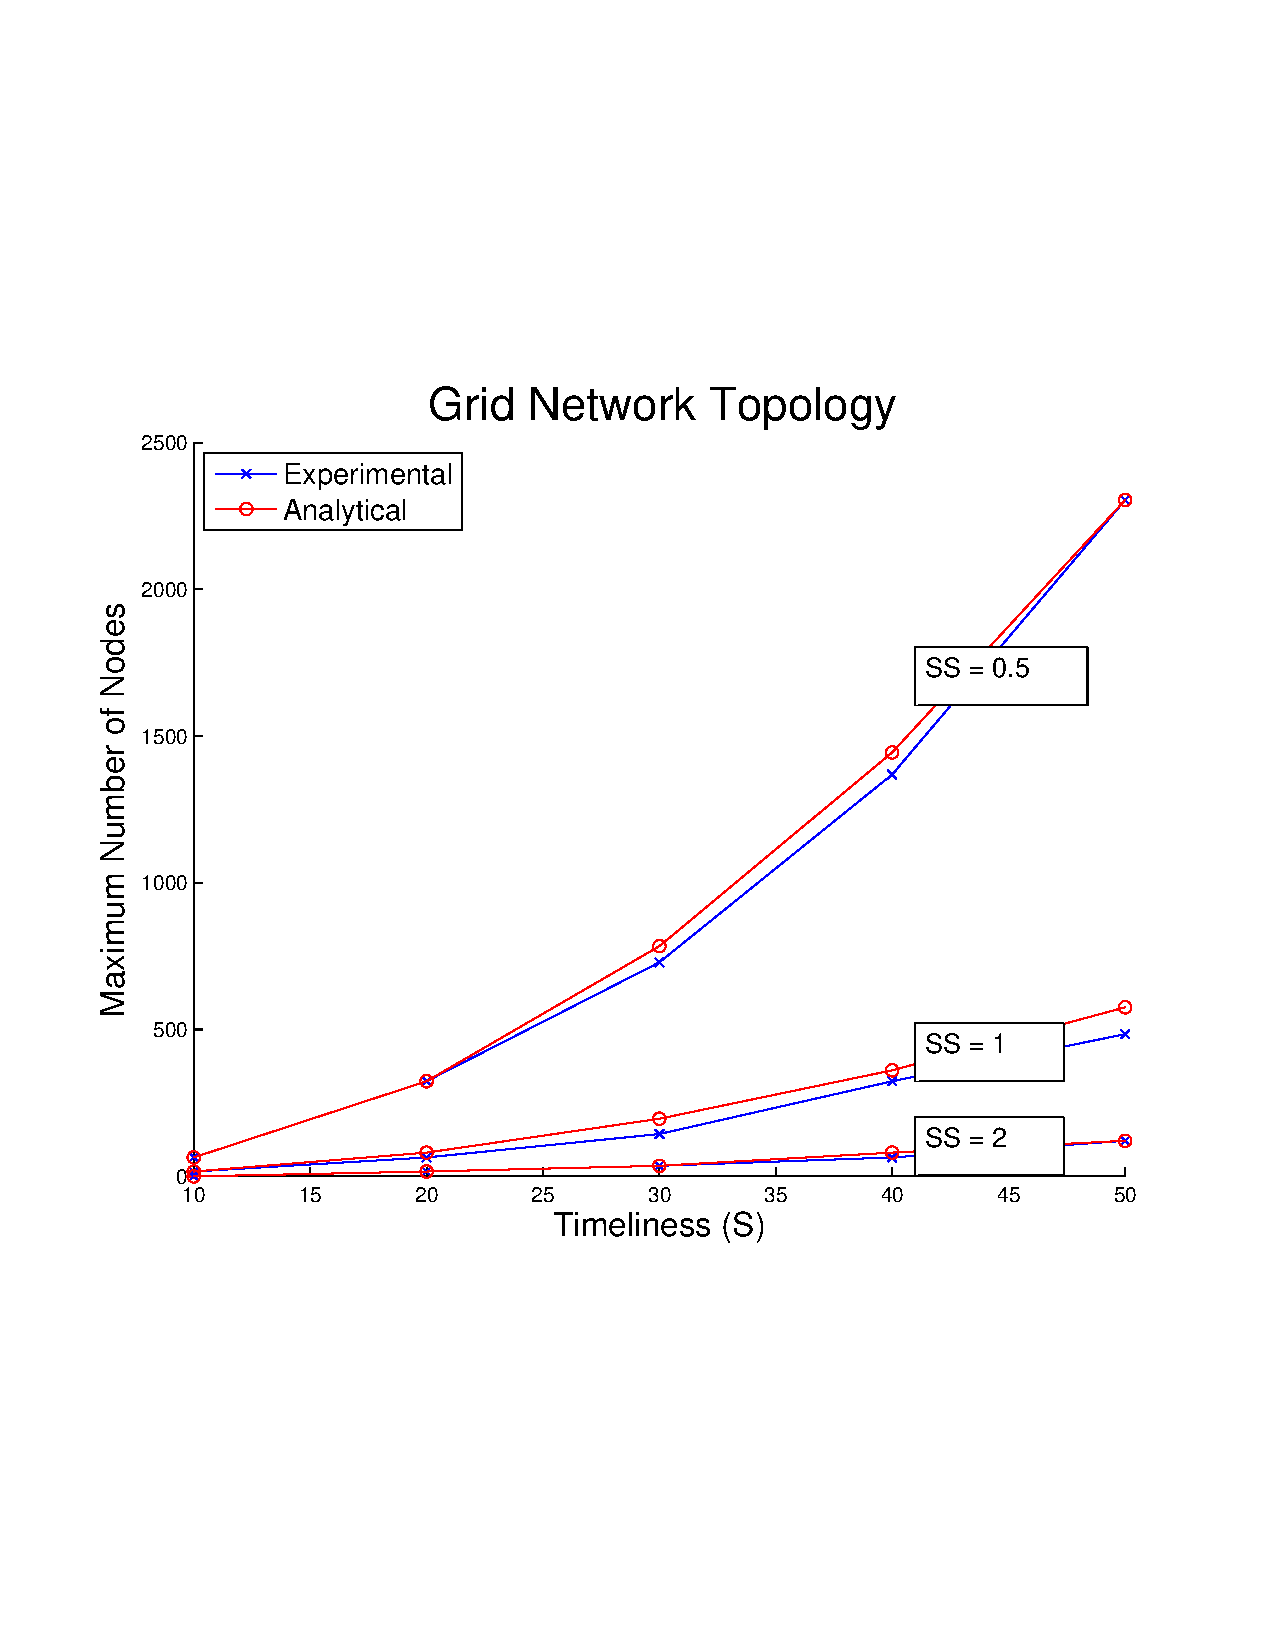
\includegraphics[scale=0.29, clip=true, trim=15mm 65mm 20mm 65mm]{grid_uni_2d_mhop_2.pdf}
        \label{fig:scal_vs_qoi_grid}
        }

   \caption{Empirical results match analytical results closely for all performed tests.  Results for each topology and a variety of sum similarity (SS) and timeliness requirements are provided.}
   \label{fig:scal_vs_qoi}

\vspace{-6mm}
\end{figure*}

\subsection{Example of Applying Framework}
\label{sec:example_apply_fw}

We illustrate the application of network signatures to the relationship in (\ref{eq:general_scal}) using an $N$-node TDMA network with three different topologies: clique, line, and grid, also known as a ``Manhattan grid.'' (Discussion of other network control protocols and topologies are addressed in Section \ref{sec:discussion}.)  We adopt a traffic model that uses Top-K queries as an example application.  We assume that all nodes have a set of collected images that are used to respond to Top-K queries.  Each node produces a query with a target image and target QoI, $\mathbf{q} = \{C, T\}$, describing the required completeness (here, we use sum similarity) and timeliness, and sends it to another node chosen at random.  The queried node will respond with the number of images, $k_{req}$, required to achieve the target sum similarity.  Values for $k_{req}$ are taken from the empirical relation in Figure \ref{fig:topkSumSim}\footnote{This application is not necessarily intended to model a known operational scenario, only a generic example to illustrate our model in a simple manner.}.  

\begin{table}[h]
\centering
\begin{tabular}{l|l|l|l|l|}
\cline{2-5}
                            					 & \textbf{CF}  					& \textbf{TF}   				& \textbf{DF}	& \textbf{PL} 			\\ \hline
\multicolumn{1}{|l|}{\textbf{Clique}} 	& N-1 							& 1                              		& 1  			& 1 					\\ \hline
\multicolumn{1}{|l|}{\textbf{Line}}   	& 3   							& $\frac{(N-1)^2}{2(N-2)}$ 	& 1.5 			& $\frac{N}{4}$			\\ \hline
\multicolumn{1}{|l|}{\textbf{Grid}}   	& 5   							& $\sqrt{N}$                       	&  2.5			& $\frac{2}{3} \sqrt{N}$   \\ \hline
\end{tabular}
\caption{CF, TF, DF, and PL values for example topologies}
\label{table:rf_ff_sf_values}
\vspace{-5mm}
\end{table}

Since our goal is to determine the point at which an average flow is no longer sustainable, we derive and use average values for $TF$, $CF$, $DF$, and $PL$ for the network.  In the case of $TF$, we use the value for the node with the largest expected $TF_i$ since flows that are routed through this node are expected to experience that largest delay and are likely to be the first that fail to meet their timeliness requirements.  Values for this example are shown in Table \ref{table:rf_ff_sf_values}, and a derivation of $TF$ for a grid network is included in Appendix \ref{sec:grid_tf_proof}.  Details about deriving the other values are explained in detail in \cite{symptotics_tech_report}.  The following equations can be used to determine QoI and network size limitations, which will be exemplified in the next two sections:

\vspace{3mm}
\noindent
Clique:
\begin{equation}
\label{eq:clique_gen}
	W \cdot T - I_S \cdot k_{req} \cdot (N-1) \geq 0
\end{equation}
Line:
\begin{equation}
\label{eq:line_gen}
	W \cdot T - 3 \cdot I_S \cdot k_{req} \cdot \frac{(N-1)^2}{N-2} - 1.5 \cdot P_S \cdot (\frac{N}{4}-1) \geq 0
\end{equation}
Grid:
\begin{equation}
\label{eq:grid_gen}
	W \cdot T - 5 \cdot I_S \cdot k_{req} \cdot \sqrt{N} - 2.5 \cdot P_S \cdot (\frac{2}{3}\sqrt{N} - 1) \geq 0
\end{equation}




\section{Validation}
\label{sec:validation}

\begin{figure}[]
\centering
       \subfigure[Line Network, $I_S = 3 MB$]{
        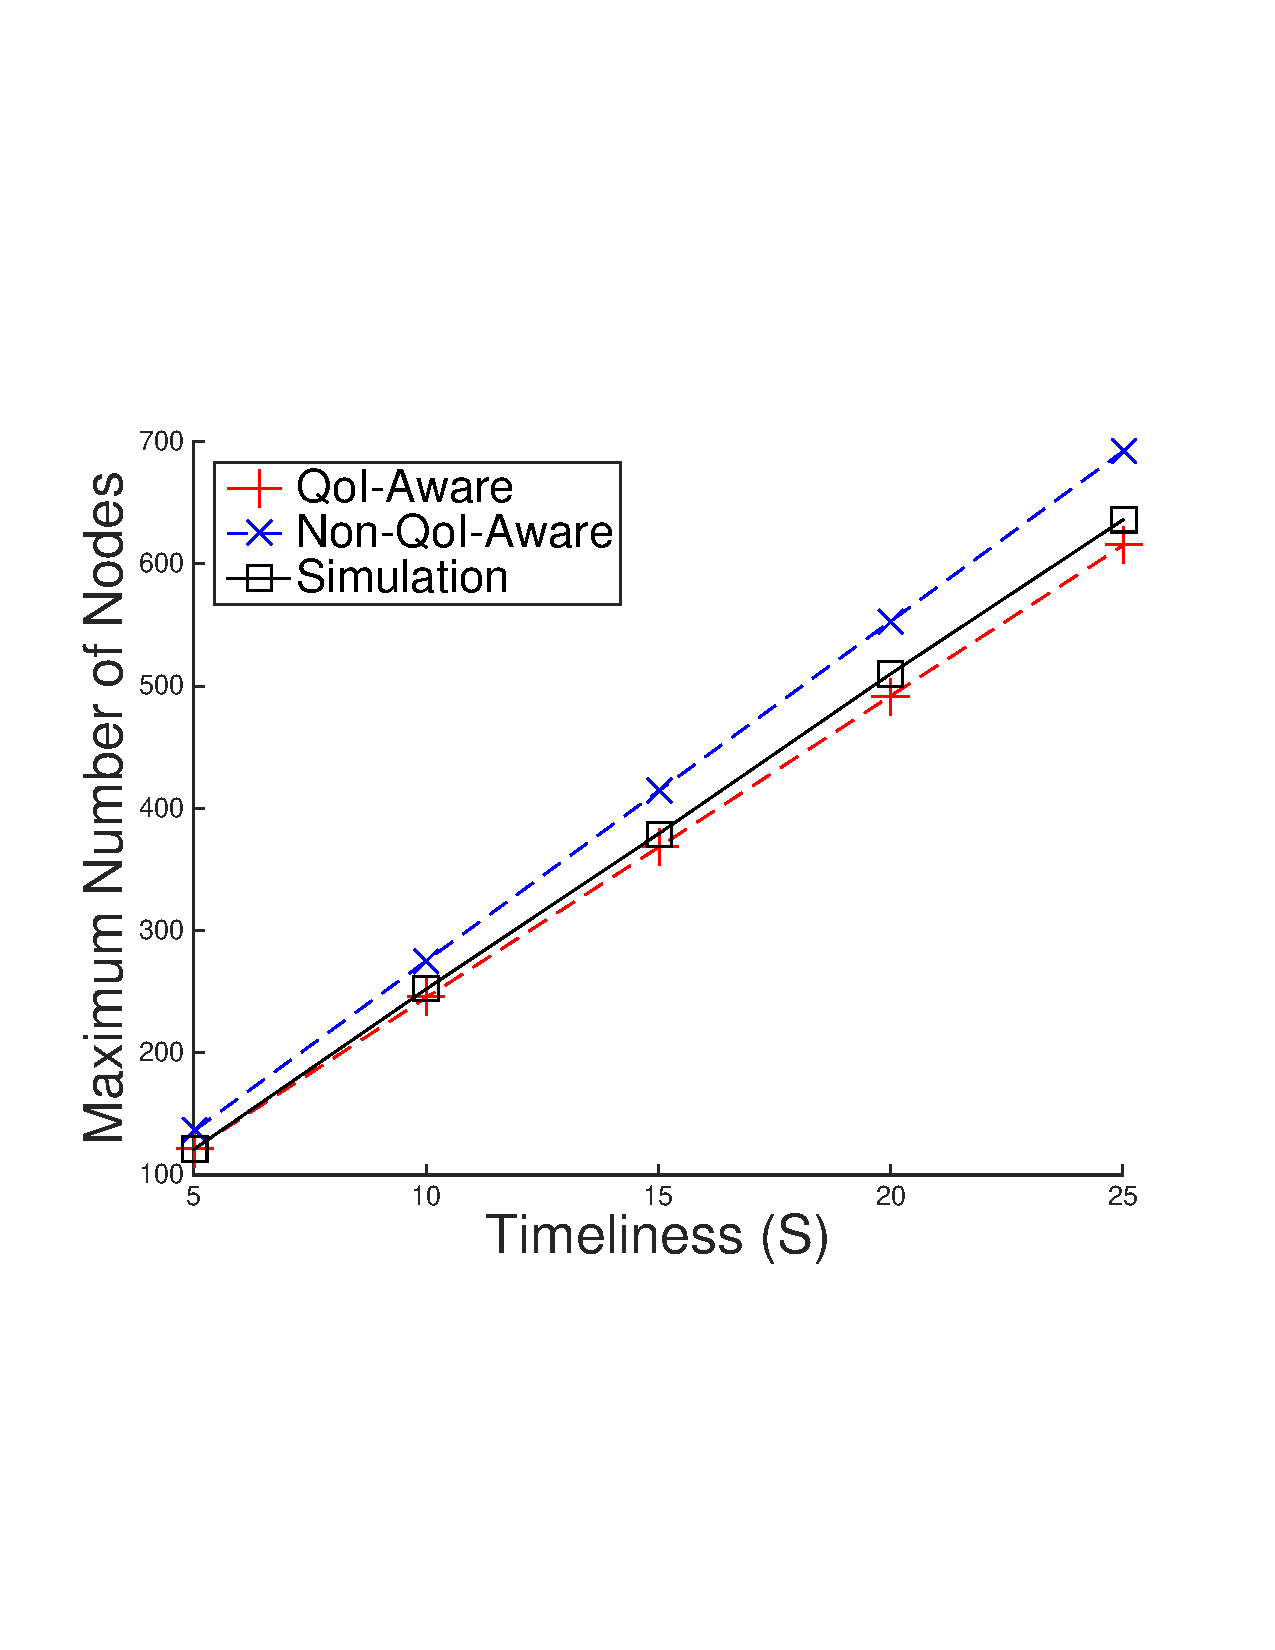
\includegraphics[scale=0.20, clip=true, trim=15mm 65mm 20mm 65mm]{figures/scal_sim_results/color_2d/line_uni_2d_qoi_vs_non_color_1.pdf}
        \label{fig:scal_vs_qoi_line}
        }
    \subfigure[Grid Network, $I_S = 6 MB$]{
        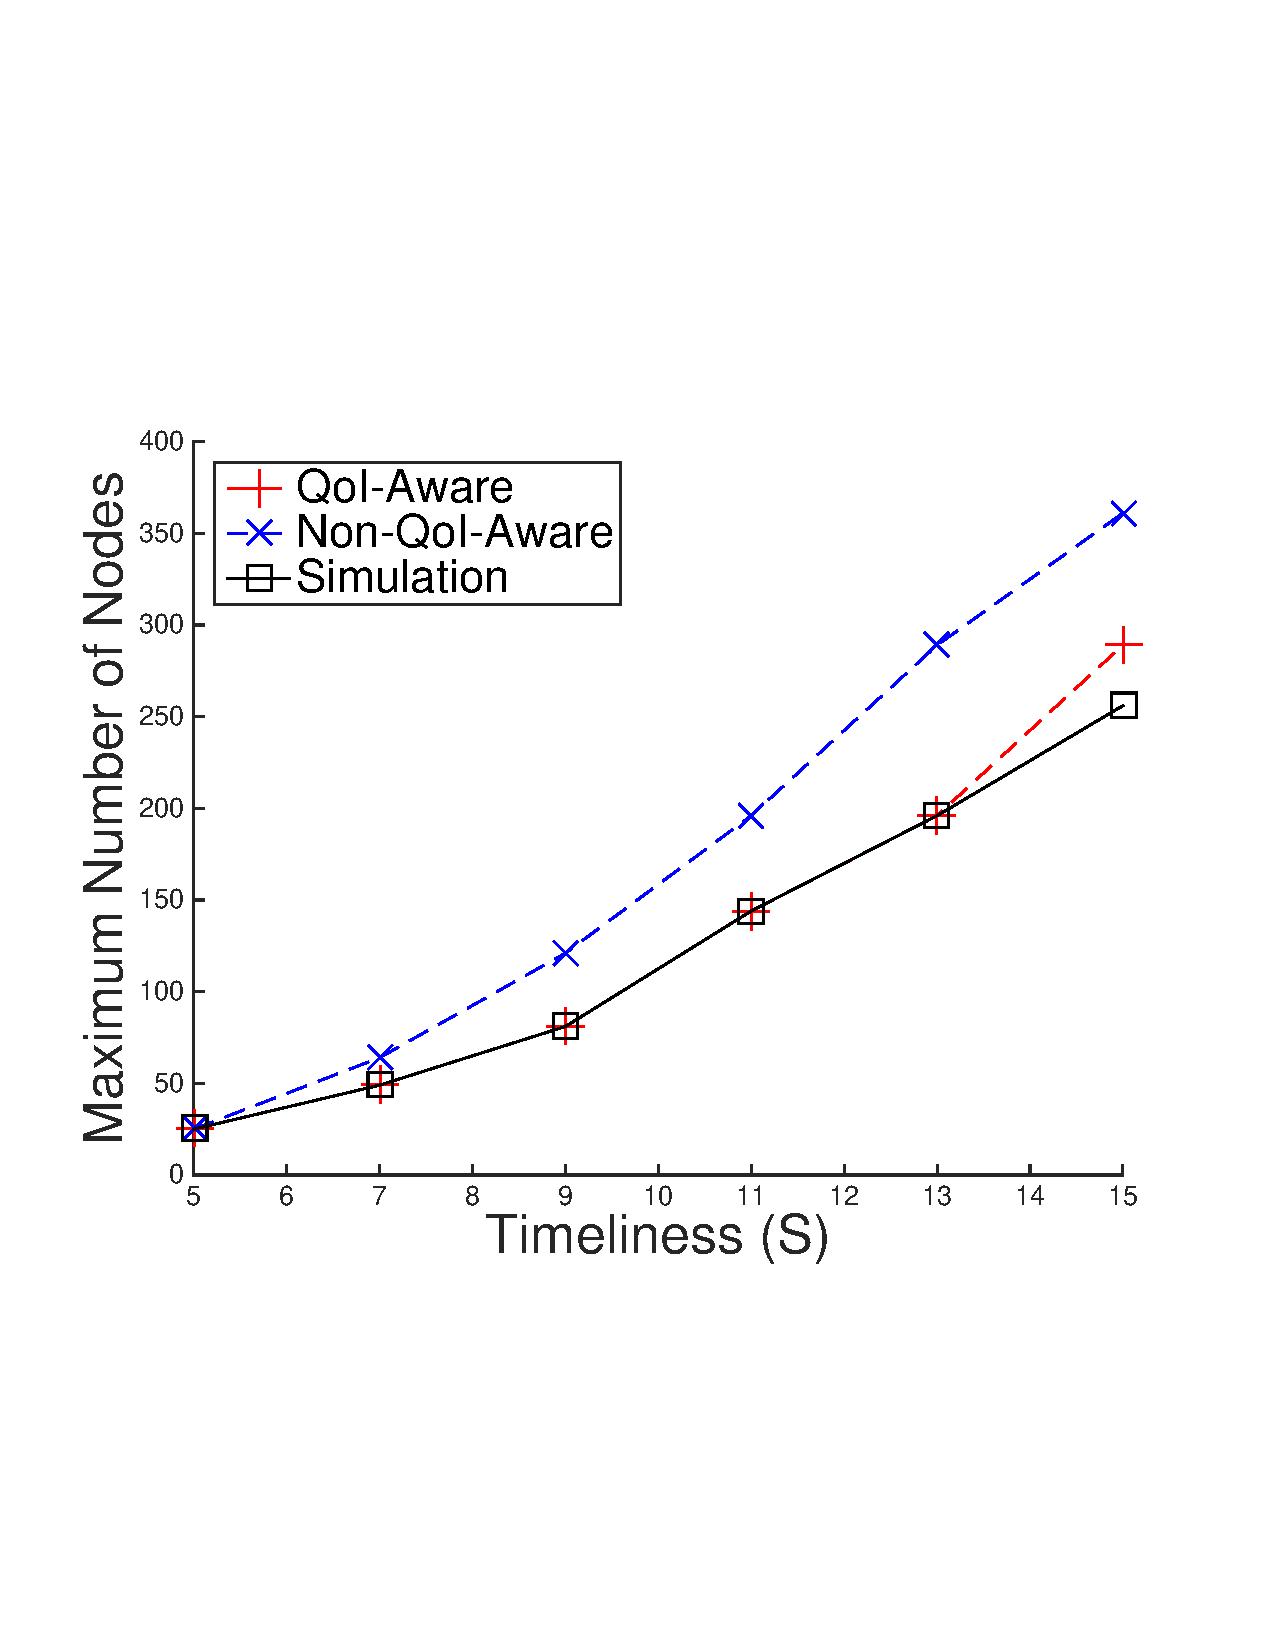
\includegraphics[scale=0.20, clip=true, trim=15mm 65mm 20mm 65mm]{figures/scal_sim_results/color_2d/grid_uni_2d_qoi_vs_non_color_3.pdf}
        \label{fig:scal_vs_qoi_grid}
        }
   \caption{Empirical results match analytical results closely for all performed tests.  Comparison to non-QoI-Aware models also show value of framework.}
   \label{fig:scal_vs_qoi}
%\vspace{-6mm}
\end{figure}

To show how effective estimates using this framework can be, we simulated the network topologies and traffic described above in Section \ref{sec:example_apply_fw} in the ns3 network simulator, comparing empirical results to those generated analytically.  To show the role of considering QoI, we also include \emph{non-QoI-Aware} scalability estimates that arise from using the scalability framework in \cite{symptotics_framework_scalability}.  We only show a subset of results in Figure \ref{fig:scal_vs_qoi} to provide evidence of the effectiveness of the methodology.  All results generated, however, exhibit very similar trends of proximity between empirical and the analytical values.

%We use a channel rate of $W= 2 Mbps$, packet sizes of $P_s = 1500$ bytes, and image sizes of 9, 12, and 48 Mbytes.  As above, the correlation between Sum Similarity and $k_{req}$ is taken from the actual observed relation in Figure \ref{fig:topkSumSim}.  All values of parameters ($SS$, $T$, $I_S$, etc.) were chosen to test a variety of network sizes and QoI requirements while remaining within realistic network sizes, both with respect to real-world deployments and simulations with feasible run-times.

%Figure \ref{fig:scal_vs_qoi} shows the maximum scalability projected by solving inequalities (\ref{eq:clique_gen})-(\ref{eq:grid_gen}) and the maximum scalability observed in our experiments.  In our simulations, we defined \emph{scalable} as a network in which all of the requested queries were entirely fulfilled within the specified timeliness requirement.  Small differences arise due to average values being used for $CF$, $TF$, $DF$, and $PL$, but, as the graphs show, in all of these scenarios, our network size estimates are very close to those realized in practical simulations.


%\begin{figure*}[]
%\centering
%    \subfigure[Clique Network, $I_S = 9 MB$]{
%        \includegraphics[scale=0.29, clip=true, trim=15mm 65mm 20mm 65mm]{figures/scal_sim_results/clique_uni_2d.pdf}
%        \label{fig:scal_vs_qoi_clique}
%        }
%    \subfigure[Line Network, $I_S = 12 MB$]{
%        \includegraphics[scale=0.29, clip=true, trim=15mm 65mm 20mm 65mm]{figures/scal_sim_results/line_uni_2d_mhop_2.pdf}
%        \label{fig:scal_vs_qoi_line}
%        }
%    \subfigure[Grid Network, $I_S = 48 MB$]{
%        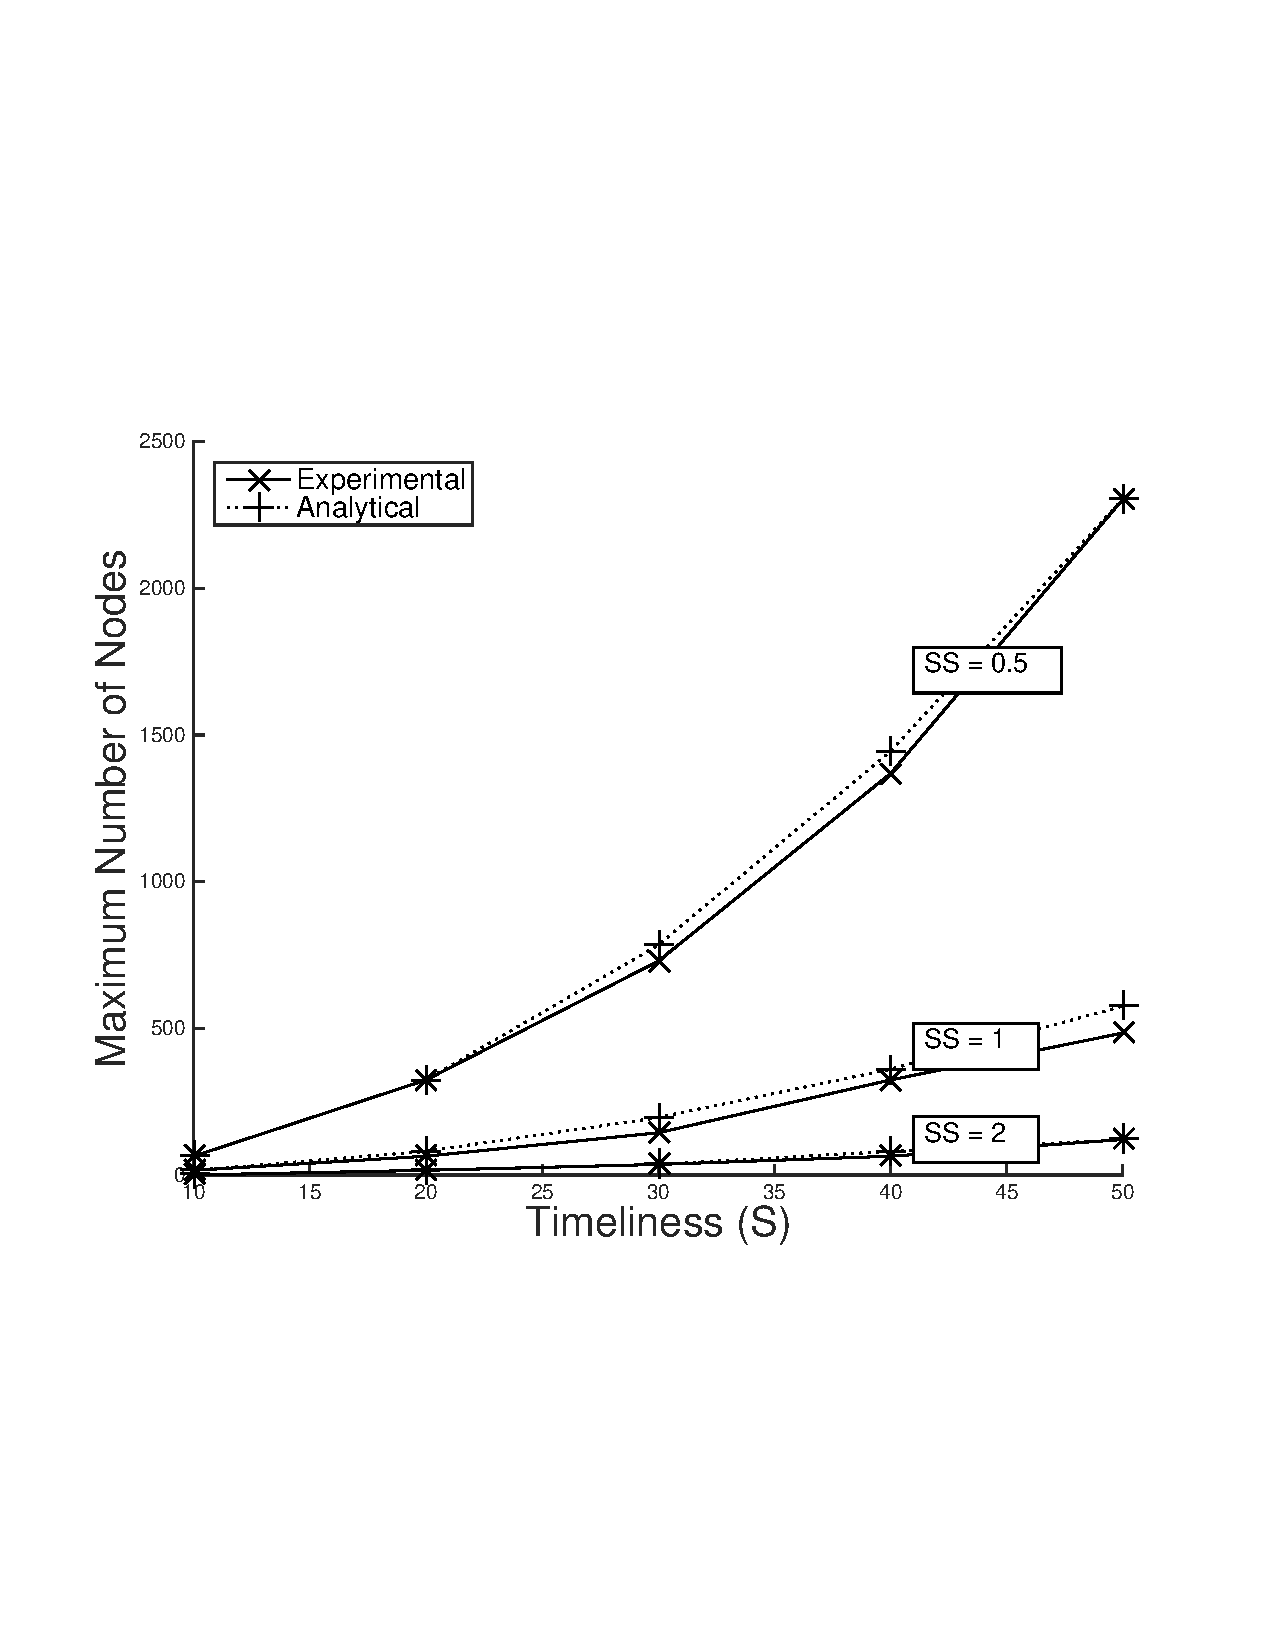
\includegraphics[scale=0.29, clip=true, trim=15mm 65mm 20mm 65mm]{figures/scal_sim_results/grid_uni_2d_mhop_2.pdf}
%        \label{fig:scal_vs_qoi_grid}
%        }
%   \caption{Empirical results match analytical results closely for all performed tests.  Results for each topology and a variety of sum similarity (SS) and timeliness requirements are provided.}
%   \label{fig:scal_vs_qoi}
%\vspace{-6mm}
%\end{figure*}

\section{Impact on Network Design}
\label{sec:network_design}

\begin{figure*}
\centering
    \subfigure[Max Timeliness vs. Network Size (Sum Sim. = 5.0)]{
	\includegraphics[scale=0.22, clip=true, trim=14mm 65mm 25mm 65mm]{tness_vs_num_nodes_5_SS_12_IS_2_W.pdf}
        \label{fig:use_case_tness_vs_num_nodes}
        }
    \subfigure[Max Sum Sim. vs. Network Size (Timeliness = 50)]{
	\includegraphics[scale=0.22, clip=true, trim=14mm 65mm 25mm 65mm]{sum_sim_vs_num_nodes_50_T_12_IS_2_W.pdf}
        \label{fig:use_case_sum_sim_vs_num_nodes}
        }
  \subfigure[Max Network Size vs. Sum Sim. (Timeliness = 10)]{
	\includegraphics[scale=0.22, clip=true, trim=14mm 65mm 25mm 65mm]{num_nodes_vs_sum_sim_10_T_12_IS.pdf}
        \label{fig:use_case_num_nodes_vs_qoi}
        }
  \subfigure[Max Network Size vs. Timeliness (Sum Sim. = 5.0)]{
	\includegraphics[scale=0.22, clip=true, trim=14mm 65mm 25mm 65mm]{num_nodes_vs_tness_5_SS_12_IS.pdf}
        \label{fig:use_case_num_nodes_vs_qoi_2}
        }

   \caption{Varying design parameters provide immediate limitations as well as evident trends and comparisons.}
   \label{fig:huh_net_design}
   \vspace{-5mm}
\end{figure*}
 
Now that we have established a model for QoI satisfiability and scalability and shown its accuracy in predicting estimated limits, we show how it can also provide quick, but useful intuition about the impact of various network parameters.  In this section, we approximate where appropriate like in (\ref{eq:tness_line_1})-(\ref{eq:tness_line}) below since the insights we seek here are more easily gained with simpler expressions, and are not greatly affected for large values.  In applying the framework in practice, though, numerical solvers can be used, removing the need for approximation.    

Throughout this section, channel rate and packet size values are again fixed at $W = 2$ Mbps and $P_S = 1,500$ Bytes.  Also, we again choose sum similarity as the illustrative metric of completeness, but any other definition of completeness could be swapped in here.  Specific values of $SS$, $T$, and $N$ are varied to show various effects, so their values are explicitly listed in each figure and/or description.

\subsubsection{Timeliness}
Since $\mathbf{q}$ is a composite requirement of both timeliness and sum similarity, the value representing completeness in this application, we can explore the limits and impact of network parameters on each separately.  First, we will substitute appropriate values for each topology, and then solve the inequality for $T$. The result for each is as follows:

\vspace{4mm}
\noindent
Clique:
\begin{equation}
	T \geq \frac{B}{W} \cdot (N -1) + \frac{P_S}{W}
\label{eq:tness_clique}
\end{equation}
Line:
\begin{eqnarray}
\label{eq:tness_line_1}
	T &\geq& 1.5 \cdot \frac{B}{W} \cdot \frac{(N-1)^2}{N-2} + 1.5 \cdot \frac{P_S}{W} \cdot (\frac{N}{4} - 1) \\
	&\approx& 1.5 \cdot \frac{B}{W} \cdot (N-1) + 1.5 \cdot \frac{P_S}{W} \cdot (\frac{N}{4} - 1)
\label{eq:tness_line}
\end{eqnarray}
%\begin{equation}
%	T \geq 1.5 \cdot \frac{B}{W} \cdot \frac{(N-1)^2}{N-2} + 1.5 \cdot \frac{P_S}{W} \cdot (\frac{N}{4} - 1)
%\label{eq:tness_line}
%\end{equation}
Grid:
\begin{equation}
	T \geq 5 \cdot \frac{\sqrt{N}}{W} \cdot (B + \frac{P_S}{3})
\label{eq:tness_grid}
\end{equation}

Using these inequalities, not only can network designers gain estimates of maximum timeliness constraints satisfiable in various network scenarios, but they can also quickly compare the dependency on specific parameters.  By quick examination of these relationships, one can see that timeliness has a $O(N)$ relationship with respect to network size in clique and line topologies, but $O(\sqrt{N})$ in a grid topology.  Figure \ref{fig:use_case_tness_vs_num_nodes} reinforces this lesson.  The graph shows minimum $T$ values for increasing values of $N$ with all other values fixed, showing that a grid network can serve tighter timeliness constraints than other topologies in larger networks.

While it may have been intuitive that a grid network should be able to serve flows with lower timeliness constraints than a line network since it will have shorter average path lengths, what is not intuitive is \emph{how much} lower of a timeliness constraint is satisfiable.  For example, we see here that a grid network can scale up to over $250$ nodes while supporting flows with $T = 40$.  A line network, on the other hand, can only scale to only approximately $20\%$ of that network size for the same timeliness value.  In either case, it is intuitive to know how a clique network's timeliness satisfiability should respond to either a grid or line network since its operation is quite different.  With the inequalities in (\ref{eq:tness_clique})-(\ref{eq:tness_grid}), though, it is quickly and easily understood.

%\begin{figure}[ht]
%\centering
%\subfigure[Achievable Timeliness vs. Network Size for a fixed Sum Similarity = 5.0]{
%	\includegraphics[scale=0.31, clip=true, trim=15mm 65mm 20mm 65mm]{figures/use_cases_examples/tness_vs_num_nodes_5_SS_12_IS_2_W.pdf}
% 	\label{fig:use_case_tness_vs_num_nodes}
%	}
%\subfigure[Achievable Sum Similarity vs. Network Size for a fixed Timeliness = 50]{
%	\includegraphics[scale=0.31, clip=true, trim=15mm 65mm 20mm 65mm]{figures/use_cases_examples/sum_sim_vs_num_nodes_50_T_12_IS_2_W.pdf}
%	\label{fig:use_case_sum_sim_vs_num_nodes}
%	}
%\caption{Achievable QoI values are quickly evident for various network sizes and comparisons between topologies are easily made.}
%\vspace{-2mm}
%\end{figure}
%
%\begin{figure}[ht]
%\centering
%  \subfigure[Varying Sum Similarity (T = 10)]{
%	\includegraphics[scale=0.31, clip=true, trim=15mm 65mm 20mm 65mm]{figures/use_cases_examples/num_nodes_vs_sum_sim_10_T_12_IS.pdf}
%	}
%  \subfigure[Varying Timeliness (SS = 5.0)]{
%	\includegraphics[scale=0.31, clip=true, trim=15mm 65mm 20mm 65mm]{figures/use_cases_examples/num_nodes_vs_tness_5_SS_12_IS.pdf}
%	}
%\caption{Achievable Network Size for Varying QoI Requirements}
% \label{fig:use_case_num_nodes_vs_qoi}
%    \vspace{-7mm}
%\end{figure}

\subsubsection{Sum Similarity (Completeness)}

In the exact same manner, we can evaluate maximum sum similarity values, $SS$, achievable by a network.  To do so, we define the inverse of the function $Q(SS) = k_{req}$ defined above.  Here, $Q'(k_{req}) = SS$ provides the sum similarity corresponding to the number of images served in each flow.  The relationship for sum similarity for each topology is described with the following relations:

\vspace{4mm}
\noindent
Clique:
\begin{equation}
	SS \leq Q'( \frac{W \cdot T - P_S}{I_s \cdot (N-1)} )
\end{equation}
Line:
\begin{equation}
	SS \leq Q'( \frac{W \cdot T - 1.5 \cdot P_S \cdot (\frac{N}{4} - 1)}{3 \cdot I_s \cdot \frac{(N-1)^2}{2(N-2)}} )
\end{equation}
Grid:
\begin{equation}
	SS \leq Q'( \frac{W \cdot T - 2.5 \cdot P_S \cdot (\frac{2}{3} \cdot \sqrt{N} - 1)}{5 \cdot I_s \cdot \sqrt{N}} )
\end{equation}

Figure \ref{fig:use_case_sum_sim_vs_num_nodes} visualizes these sum similarity limits for network instances of different numbers of nodes while timeliness is fixed.  Here, again, limits and trends are quickly evident.  In addition, the nonlinearity of completeness requirements are manifested here as the data requirements for the highest completeness requirements are only sustainable for small networks, but as the network size increases, the impact on achievable completeness is not as dramatic.  

To highlight this example, we can refer back to Figure \ref{fig:topkAvgNumSameSet} and see that in order to obtain $7$ images matching the target image on average, we should collect $~28$ images, which we see from \ref{fig:topkSumSim} equates to a sum similarity of approximately $6.5$.  If we require a timeliness of $50$ seconds and our network topology has $50$ nodes that are in a line, a sum similarity of $6.5$ is the maximum completeness the network can support.  If these same nodes are arranged in a grid network, however, we see that the network still has the capability to support more traffic, closer to a sum similarity of $11.5$, which is twice as many images on average.
 
\subsubsection{Scalability}

Finally, given a topology and application with predetermined requirements of $\mathbf{q}$, we may be simply interested in how large our network can grow before its capacity to deliver the desired QoI is no longer possible.  The proper relationships to answer this question are below in (\ref{eq:scal_clique})-(\ref{eq:scal_grid}), and Figure \ref{fig:use_case_num_nodes_vs_qoi} gives maximum scalability examples when either component of $\mathbf{q}$ is varied.  Once again, the graphs show the major impact completeness and timeliness requirements can have on network size.

\vspace{4mm}
\noindent
Clique:
\begin{equation}
	N \leq \frac{W \cdot T - P_S}{B} -1
\label{eq:scal_clique}
\end{equation}
Line:
%\begin{equation}
%	W \cdot T - 3 \cdot B \cdot \frac{(N-1)^2}{2(N-2)} - 1.5 \cdot P_S \cdot (\frac{N}{4} - 1)
%\end{equation}
%\indent which can be approximated to:
\begin{equation}
	N \leq \frac{W \cdot T + \frac{3}{2}P_S}{\frac{3}{2}B+\frac{3}{8}P_S}
\label{eq:scal_line}
\end{equation}
Grid:
\begin{equation}
	N \leq (\frac{W \cdot T}{5 \cdot B + \frac{5}{3} \cdot P_S})^2
\label{eq:scal_grid}
\end{equation}




\section{Scalably Feasible QoI Regions}
\label{sec:scal_feasible_qoi}

Now let us consider a special case where nodes collect a total of $k_{req}$ images, but each image must come from a different node, perhaps because each node only has one image or maybe by design to provide increased credibility through corroboration, another contextual metric of interest in QoI-aware networks. This scenario allows us to illustrate an interesting observation.  

Consider a set of QoI requirements that include completeness and timeliness, $\mathbf{q} = \{C,T\}$.  As previously noted, a certain number of images are required to achieve this desired level of completeness, $Q(C) = k_{req}$.  Unlike the model used in Section \ref{sec:network_design}, however, each node can contribute only one image to $k_{req}$, which implies a minimum network size of $N \geq k_{req}$ in order to achieve the completeness outlined in the QoI requirements.  On the other hand, applying the framework of Section \ref{sec:qoi_scalability} to this network, we can determine the maximum network size, which we will call $N_{max}$ here for distinction.  

These two facts are important, because when $N_{max} < k_{req}$, then it is not possible to provide the QoI level $\mathbf{q}$.  Hence, we say that this set of QoI requirements is infeasible, or \emph{scalably infeasible}.  This phenomenon defines the concept of a \emph{Scalably Feasible QoI Region}, which refers to the region in which all sets of QoI pairs can be supported with the given network signature.  

\vspace{-4mm}
\begin{figure}[ht]
\centering
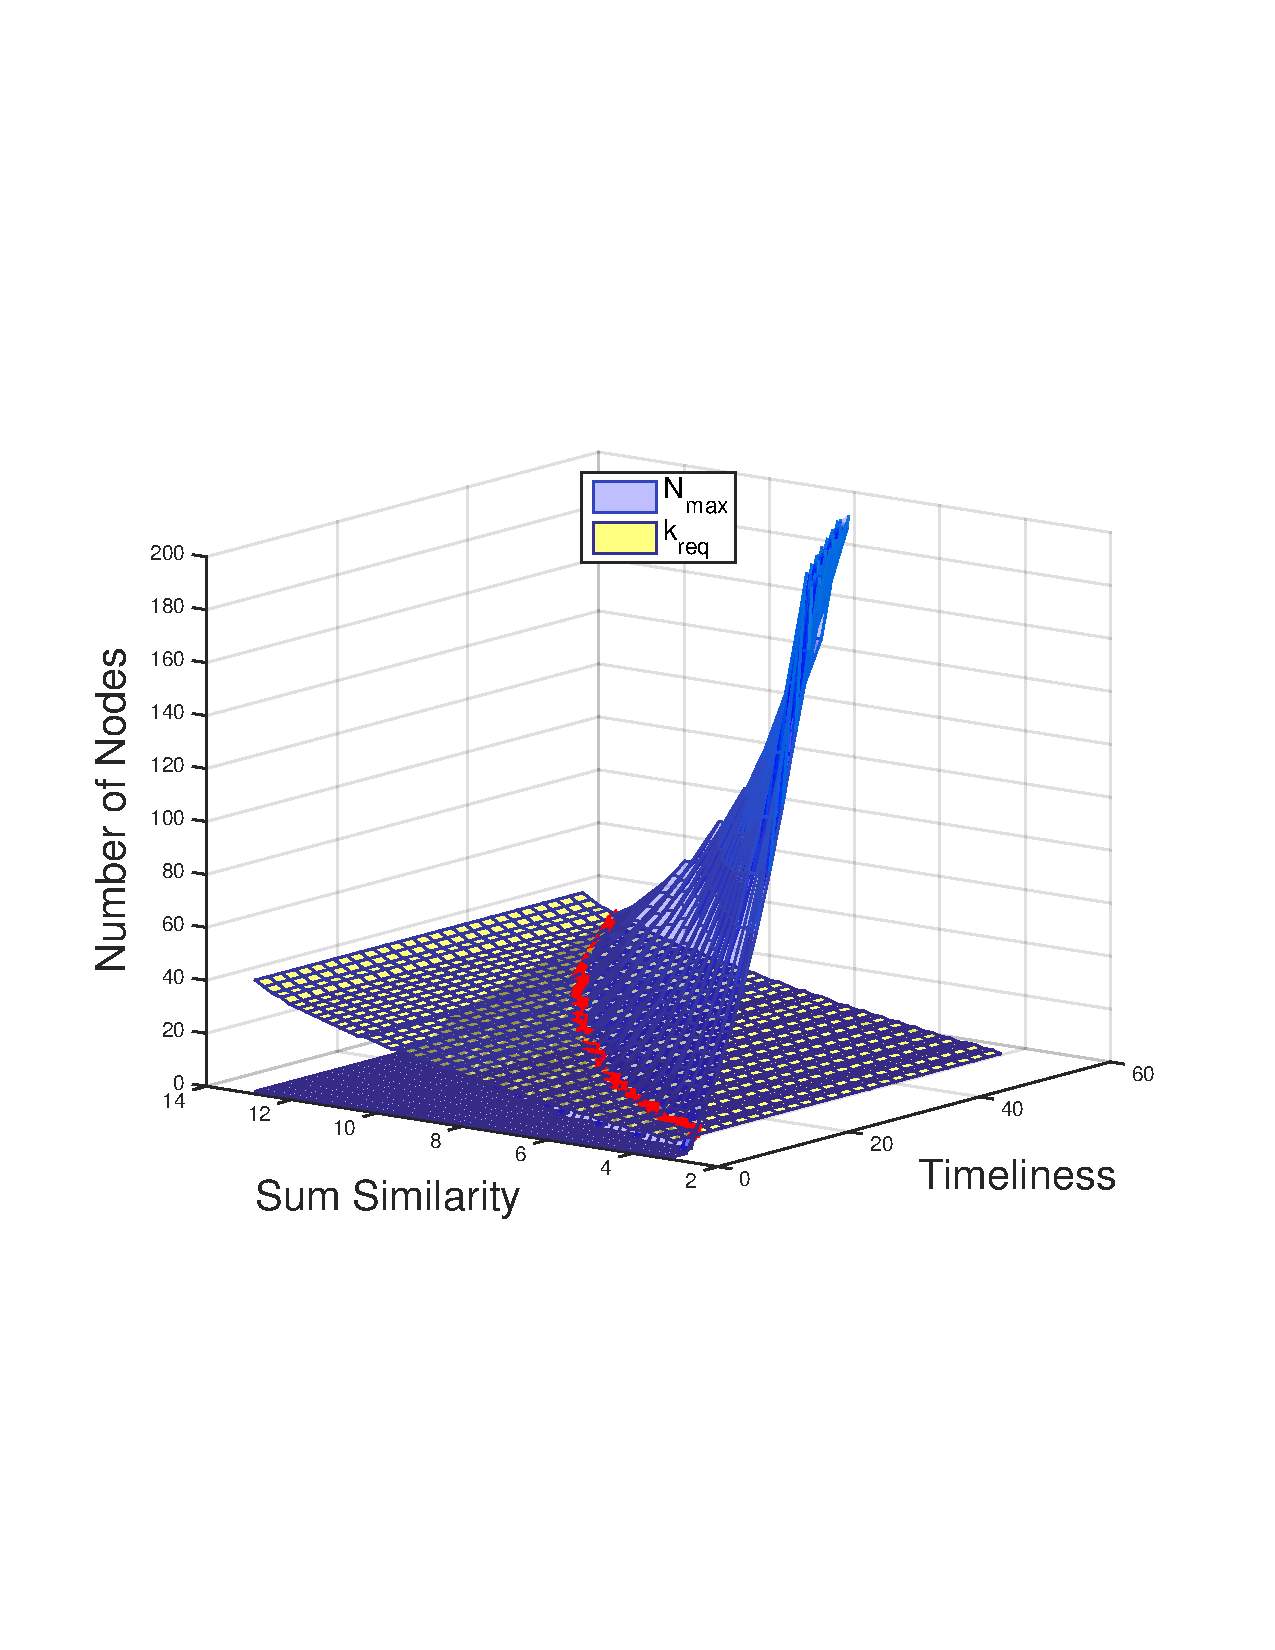
\includegraphics[scale=0.31, clip=true, trim=10mm 65mm 20mm 77mm]{scal_feas_qoi_region_3d_plot_3.pdf}
\vspace{-5mm}
\caption{The blue plane represents maximum scalability, and the yellow plane represents minimum required images.  Therefore, all {Sum Similarity, Timeliness} pairs to the right of the red line are within the scalably feasible QoI region.}
 \label{fig:scal_feasible_region}
 \vspace{-3mm}
\end{figure}

Figure \ref{fig:scal_feasible_region} provides a visual representation of this region for a grid network that institutes the given traffic model assuming traffic is routed over randomly chosen shortest-path routes.
%\footnote{Details of applying the framework are omitted due to space constraints.}.  
Here, $N_{max}$, calculated for $\mathbf{q}$ pairs from $\{2.5,1\}$ to $\{13.0, 50\}$, is shown in the graph by the blue surface.  On the same graph is the number of images required, $k_{req}$, for each Sum Similarity requirement, shown with the yellow surface on the graph.  The intersection of these two surfaces, displayed with a red line, provides the edge of the scalably feasible QoI region.  In this example, all sum QoI pairs to the right of this line, i.e. the region where $N_{max} > k_{req}$, are scalably feasible.  

In general, regardless of how many images a node has, it is possible to analyze the trade-off between different QoI attributes for a fixed value of maximum network size, $N_{max}$.  Specifically, by fixing $N$ in (\ref{eq:clique_gen})-(\ref{eq:grid_gen}), one can obtain $T$ and $k_{req}$ (and, hence, $C$) resulting in the set of supportable $\{C,T\}$ pairs defining a feasible region for QoI. This region can be visualized by intersecting the blue scalability curve with a flat surface fixed at $N_{max}$ instead of the yellow surface in Figure \ref{fig:scal_feasible_region}.  The scenario given in this section goes one step further and also takes into account  the network size actually required to generate/support a given QoI requirement (using the non-flat yellow surface derived from experimental results in Figure \ref{fig:scal_feasible_region}).


\section{Discussion}
\label{sec:discussion}

%Given the coarseness of the model and the abstraction of many details, we note that the above is not a perfect predictor of a real network's capabilities. However, we show with packet-based, multi-hop simulation results in Section \ref{sec:validation}, that our approach is very accurate in practice.  
%Furthermore, the framework presented is more than accurate enough to expose tradeoff points in QoI and scalability as shown in Section \ref{sec:network_design}.  

We note that although TDMA is primarily used in this work, the same approach can be taken to derive QoI-based relations in networks that use other MAC layer protocols.  In these cases, the appropriate Delay Factor would need to be derived for each protocol.  To examine an 802.11 network, for example, the $DF$ would capture queuing delays and could be determined by extending a delay model such as in \cite{perf_anal_80211_lan_mac}, for example.  

Similarly, although we only address the regular topologies of clique, line, and grid networks here, we believe the framework can be applied to more complex, irregular network topologies.  In fact, some of the simple models presented here may already be quite useful for some of the topologies addressed.  As shown in \cite{symptotics_tech_report}, for example, a dense random network may be closely approximated by a clique network, or random networks' capabilities can be approximately bounded by the limits of clique and grid networks, since these networks can be viewed of as examples of dense and sparse random networks, respectively.  

Another approach to more complex topologies is to extract expressions for $DF$, $TF$, etc. empirically from simple simulations when deriving closed-form expressions is impossible or infeasible.  This approach would provide the benefits of the framework presented here without being as complicated as a packet-based simulation or testbed that must implement all layers of the network.  We are currently pursuing realistic examples and validation of this concept for more complex networks, including random and social network topologies among others. 

%As \cite{symptotics_tech_report} shows, though, the simple models studied here are already useful for some topologies not explicitly addressed.  For example, a dense random network may be closely approximated by a clique network, or, as validated with simulations in \cite{symptotics_tech_report}, random networks' capabilities can be approximately bounded by the limits of clique and grid networks, since these networks can be viewed of as examples of dense and sparse random networks, respectively.  



\section{Conclusion}
\label{sec:conclusion}

Wrap it up with the highlights/takeaways.  Maybe also include future work.

\appendices

%\section{Explanation of Expected QoI with Random Image Selection}
%\label{sec:expl_exp_qoi}
%
%\subsection{Top-K}
%First, we explain the expected number of images that are from the same set as the target image in the Top-K algorithm when images are selected from the entire image pool at random.  We define the following:  
%
%\begin{itemize}
%	\item $n$ = total number of images (summed over all sets)
%	\item $S$ = number of sets
%	\item $S_k$ = set of target image
%	\item $k$ = number of images selected
%	\item $N_{S}$ = number of images in each set (for simplicity, assumed to be the same for all sets)
%	\item $x$ = number of images returned from set $S_k$
%\end{itemize}
%
%\begin{equation}
%	P( X = x | k ) = \left\{ \,
%	\begin{IEEEeqnarraybox}[][c]{l?s}
%		\IEEEstrut
%		\frac{{k \choose x} * {n-k \choose k-x} }{ {n \choose k}} & if $k \leq N_S$, \\
%		\frac{ {N_{S} \choose x} * {n-N_{S} \choose k-x}}{{n \choose k}} & if $N_S < k \leq n-N_S$
%		\IEEEstrut
%	\end{IEEEeqnarraybox}
%	\right.
%\label{eq:prob_topk_rand}
%\end{equation}
% 
%%If $k \leq N_{S}$, then 
%%\begin{equation}
%%	p(X = x | k) = \frac{{k \choose x} * {n-k \choose k-x} }{ {n \choose k}}, \forall x \leq k
%%\end{equation}
%%Otherwise, $p(X = x | k) = 0$.
%Equation \ref{eq:prob_topk_rand} provides the probability that $x$ of the $k$ selected images will be from the target set.  When $k \leq N_S$, the total number of possible combinations of choosing $x$ from the target set and $k-x$ from the $n - N_{S_k}$ remaining images over the entire sample space ($n$ choose $k$).  
%%Naturally, we cannot end up with more images from the target set than the number of images selected, and, thus the probability of $x > k$ is zero.  
%When $N_{S} < k < n-N_{S}$, then we consider the possible combinations of choosing $x$ images from the target set and $k-x$ images from the remaining $n-N_{S}$ images.
%This probability formula can then be used to derive the expected values of $x$ displayed in Figure \ref{fig:topkAvgNumSameSet}. 
%%Finally, when $k > n-N_{S}$, then $k - (n-N_{S} + x)$ images must be from the target set by the pigeonhole principle, so the $p(X = x) = 0$ for all $k > n - N_{S} + x$.  Otherwise, the same expression as directly above is true.
%
%%\begin{equation}
%%	p(X = x | N_S < k < n - N_S) = \frac{ {N_{S} \choose x} * {n-N_{S} \choose k-x}}{{n \choose k}}
%%\end{equation}
%
%\subsection{Clustering}
%For Clustering, we want to determine the probability that we will cover each of the $S$ sets with at least one of the $k$ chosen images if we had chosen them randomly.  We will call $X_i$ the random variable that represents the number of images from set $i$ in the results.  We use the following expression:
%
%\begin{equation}
%	P( X_i > 0 , \forall i | k) = (1 - P(X_i = 0))^{S}
%\end{equation}
%where $X_i$ is given by a multivariate hypergeometric distribution, which gives us the following:
%\begin{equation}
%	P(X_i = 0 | k) = \frac{{n-N_s \choose k}}{{n \choose k}}
%\end{equation}
%
%This probability expression is plotted directly against the percentage of trials in which all sets were covered in experiments using the Clustering algorithm in Figure \ref{fig:clusterAvgNumSetsCov}.



\section{Proof of Traffic Factor for Grid Network}
\label{sec:grid_tf_proof}
We outline a simple proof for determining the traffic factor of the center node in a grid topology of $N$ nodes using ``Row-First, Column-Second" routing, not including traffic originating or ending at the center node.  For simplicity, we only go through the proof for when $\sqrt{N}$ is odd.  The construction for even values of $\sqrt{N}$ follows from the same logic.

Assume that each node is the source of exactly one flow at all times and that the destination of this flow is uniformly chosen from all other $N-1$ nodes in the network.  Node $i$, then, has a $\frac{1}{N-2}$ chance of choosing each other node that is not the center of the grid.  For each source node, we can determine the number of destinations that route through the center.  We separate nodes into two categories for this counting.

\begin{figure}
\begin{centering}
    \includegraphics[scale=0.33]{TF_proof_fig_color.pdf}
    \vspace{-4mm}
    \caption{Sources and destinations used in proving TF for grid networks}
    \label{fig:TF_proof_fig}
    \vspace{-6mm}
\end{centering}
\end{figure}

The first set of nodes we consider are those circled in set $A$ in Figure \ref{fig:TF_proof_fig}.  Through manual inspection, one can deduce that the only destination nodes in the figure that result in a path that is relayed by the center node are the two bottom nodes in the center column in the figure, marked with blue.  We define the probability of a node in set $A$ choosing one of these destinations from all possible destinations as $P_{A} = \frac{\frac{\sqrt{N}-1}{2}}{N-2}$.

Now, we can count the total number of nodes for which this probability holds.  From the figure, we can quantify the number of circled nodes, but we must also consider the reverse, i.e. imagine the figure rotated vertically, so the total number of nodes falling into set $A$ is actually $N_A = \sqrt{N} \cdot (\sqrt{N}-1)$.
Then, the expected number of paths being forwarded by the center node at any given time by nodes in set $A$ is simply the product of $P_A$ and $N_A$:
\begin{equation}
	E[TF_{A}] = \frac{\frac{\sqrt{N}-1}{2}}{N-2}  \cdot  \sqrt{N} \cdot (\sqrt{N}-1)
\end{equation}

Next, we consider the nodes not in set $A$.  These nodes are in the same row as the center node, and we will call them set $B$, also shown in Figure \ref{fig:TF_proof_fig}.  Here, all destinations on the ``opposite" side of the center as well as those in the same column of the center require being routed through the center node when originating from any nodes in set $B$.  Just as above, we can relate the probability of choosing one of these destinations as $P_{B} = \frac{\frac{\sqrt{N}+1}{2} \cdot \sqrt{N} - 1}{N-2}$.

Using the number of nodes in set $B$, $N_{B} = \sqrt{N}$, the resulting expected traffic factor for the center node attributed by nodes in set $B$ is
\begin{equation}
	E[TF_{B}] = \frac{\frac{\sqrt{N}+1}{2} \cdot \sqrt{N} - 1}{N-2} \cdot 2 \cdot (\frac{\sqrt{N}-1}{2})
\end{equation}

Since sets $A$ and $B$ account for all non-center nodes in the network, the overall expected traffic factor is just the sum of $E[TF_A]$ and $E[TF_B]$, which simplifies to
\begin{equation}
	E[TF] = \frac{\sqrt{N}(N - 2) + 1}{N-2}
\end{equation}
which is effectively $\sqrt{N}$ for large $N$.
\vspace{-1mm}





%\appendix
%\input{sections/random_explanation}
% conference papers do not normally have an appendix


% use section* for acknowledgement
%\section*{Acknowledgment}


%The authors would like to thank...


% trigger a \newpage just before the given reference
% number - used to balance the columns on the last page
% adjust value as needed - may need to be readjusted if
% the document is modified later
%\IEEEtriggeratref{8}
% The "triggered" command can be changed if desired:
%\IEEEtriggercmd{\enlargethispage{-5in}}

% references section

% can use a bibliography generated by BibTeX as a .bbl file
% BibTeX documentation can be easily obtained at:
% http://www.ctan.org/tex-archive/biblio/bibtex/contrib/doc/
% The IEEEtran BibTeX style support page is at:
% http://www.michaelshell.org/tex/ieeetran/bibtex/
%\bibliographystyle{IEEEtran}
% argument is your BibTeX string definitions and bibliography database(s)
%\bibliography{IEEEabrv,../bib/paper}
%
% <OR> manually copy in the resultant .bbl file
% set second argument of \begin to the number of references
% (used to reserve space for the reference number labels box)
%\begin{thebibliography}{1}


\bibliographystyle{unsrt}

\bibliography{references}


%\bibitem{IEEEhowto:kopka}
%H.~Kopka and P.~W. Daly, \emph{A Guide to \LaTeX}, 3rd~ed.\hskip 1em plus
%  0.5em minus 0.4em\relax Harlow, England: Addison-Wesley, 1999.

%\end{thebibliography}




% that's all folks
\end{document}


